% =====================================================================
% Natural Gas Trading Strategy - Comprehensive Analysis Report
% =====================================================================

\documentclass[12pt,a4paper]{article}

% Packages
\usepackage[utf8]{inputenc}
\usepackage[margin=1in]{geometry}
\setlength{\headheight}{14.5pt}  % Fix fancyhdr warning
\usepackage{graphicx}
\usepackage{amsmath}
\usepackage{amssymb}
\usepackage{booktabs}
\usepackage{longtable}
\usepackage{hyperref}
\usepackage{xcolor}
\usepackage{fancyhdr}
\usepackage{titlesec}
\usepackage{caption}
\usepackage{subcaption}
\usepackage{enumitem}
\usepackage{float}
\usepackage{multirow}
\usepackage{array}
\usepackage{siunitx}

% Hyperlink setup
\hypersetup{
    colorlinks=true,
    linkcolor=blue,
    filecolor=magenta,
    urlcolor=cyan,
    citecolor=blue,
    pdftitle={Natural Gas Trading Strategy Analysis},
    pdfauthor={Zaid Annigeri},
}

% Header and Footer
\pagestyle{fancy}
\fancyhf{}
\rhead{Natural Gas Trading Strategy}
\lhead{Quantitative Finance Research}
\rfoot{Page \thepage}

% Title formatting
\titleformat{\section}{\Large\bfseries}{\thesection}{1em}{}
\titleformat{\subsection}{\large\bfseries}{\thesubsection}{1em}{}

% Document begins
\begin{document}

% =====================================================================
% TITLE PAGE
% =====================================================================
\begin{titlepage}
    \centering
    \vspace*{2cm}

    {\Huge\bfseries Natural Gas Return Prediction \\ \& Trading Strategy\par}
    \vspace{0.5cm}
    {\Large A Quantitative Analysis Comparing \\ Fundamental Factors vs Time Series Models\par}

    \vspace{2cm}

    {\Large\itshape Zaid Annigeri\par}
    \vspace{0.5cm}
    {\large Master of Quantitative Finance Program\par}
    {\large Rutgers Business School\par}

    \vfill

    {\large \textbf{Abstract}\par}
    \vspace{0.5cm}
    \begin{minipage}{0.8\textwidth}
        \small
        This research compares fundamental factor analysis against time series models for predicting monthly natural gas returns. Using 71 months of data (January 2020 - November 2025), we demonstrate that a parsimonious OLS model with six fundamental factors outperforms ARMA/GARCH benchmarks by 54\% (SSR metric). Walk-forward backtesting yields a Sharpe ratio of 1.07 with 63\% directional accuracy, validating the predictive power of fundamental analysis at monthly frequency. The study highlights critical lessons in position sizing and risk management, particularly during extreme volatility periods (COVID-19 and Ukraine war).
    \end{minipage}

    \vfill

    {\large November 2025\par}
\end{titlepage}

% =====================================================================
% ONE-PAGE RESEARCH SUMMARY (Insert after title page)
% =====================================================================
% Insert this page after the title page and before table of contents
% Add: \input{One_Page_Summary.tex} after \end{titlepage}
% =====================================================================

\newpage
\thispagestyle{empty}  % No page number

\begin{center}
{\Huge\bfseries Research Summary}
\vspace{0.3cm}

{\large Natural Gas Return Prediction \& Trading Strategy}
\end{center}

\vspace{0.4cm}

% Main finding box
\noindent\colorbox{blue!10}{%
    \parbox{0.96\textwidth}{%
        \centering
        \textbf{\Large KEY FINDING} \\[0.2cm]
        {\large Fundamental factors outperform time series models by \textbf{54\%} (SSR metric) \\
        for monthly natural gas return prediction}
    }%
}

\vspace{0.4cm}

% Three-column layout for metrics
\noindent
\begin{minipage}[t]{0.31\textwidth}
    \centering
    \fcolorbox{green!50!black}{green!10}{%
        \parbox{0.9\textwidth}{%
            \centering
            \textbf{Out-of-Sample Performance}\\[0.2cm]
            \begin{tabular}{@{}ll@{}}
            Sharpe Ratio: & \textbf{1.07} \\
            Sortino Ratio: & \textbf{1.69} \\
            Win Rate: & \textbf{63\%} \\
            Total Return: & \textbf{409\%} \\
            Max Drawdown: & -59\% \\
            \end{tabular}
        }%
    }
\end{minipage}%
\hfill
\begin{minipage}[t]{0.31\textwidth}
    \centering
    \fcolorbox{orange!50!black}{orange!10}{%
        \parbox{0.9\textwidth}{%
            \centering
            \textbf{Model Comparison (SSR)}\\[0.2cm]
            \begin{tabular}{@{}lr@{}}
            OLS (6 vars): & \textbf{3.80} \\
            OLS (23 vars): & 2.57 \\
            Random Forest: & 2.79 \\
            ARMA(2,1): & 5.68 \\
            GARCH(1,1): & 5.86 \\
            \end{tabular}
            \vspace{0.1cm}

            \small \textit{Lower is better}
        }%
    }
\end{minipage}%
\hfill
\begin{minipage}[t]{0.31\textwidth}
    \centering
    \fcolorbox{purple!50!black}{purple!10}{%
        \parbox{0.9\textwidth}{%
            \centering
            \textbf{Top 3 Factors}\\[0.2cm]
            \begin{tabular}{@{}lc@{}}
            Henry Hub Spot & 53\% \\
            Net Trade Bal. & 22\% \\
            Coal Price & 21\% \\
            \end{tabular}
            \vspace{0.1cm}

            \small \textit{Variance explained}
            \vspace{0.15cm}

            \small Parsimonious model: \\
            \small \textbf{6 factors} vs 23
        }%
    }
\end{minipage}

\vspace{0.5cm}

% Methodology snapshot
\noindent\fcolorbox{black}{gray!5}{%
    \parbox{0.96\textwidth}{%
        \textbf{METHODOLOGY SNAPSHOT} \\[0.2cm]
        \begin{minipage}{0.48\textwidth}
            \textbf{Data:} \\
            • 71 months (Jan 2020 - Nov 2025) \\
            • EIA, FRED, ICE data sources \\
            • 23 initial factors → 6 significant

            \vspace{0.2cm}
            \textbf{Models Tested:} \\
            • OLS Regression (full \& parsimonious) \\
            • ARMA / GARCH time series \\
            • Random Forest ensemble
        \end{minipage}%
        \hfill
        \begin{minipage}{0.48\textwidth}
            \textbf{Validation:} \\
            • Walk-forward backtesting \\
            • 36-month expanding window \\
            • 35 out-of-sample periods \\
            • No look-ahead bias

            \vspace{0.2cm}
            \textbf{Industry Comparison:} \\
            • AQR Managed Futures: 0.40-0.60 Sharpe \\
            • Our Strategy: \textbf{1.07 Sharpe} (78\% higher)
        \end{minipage}
    }%
}

\vspace{0.4cm}

% Six significant factors
\noindent\fcolorbox{blue!50!black}{blue!5}{%
    \parbox{0.96\textwidth}{%
        \textbf{SIX STATISTICALLY SIGNIFICANT FACTORS (p < 0.1)} \\[0.2cm]
        \small
        \begin{tabular}{@{}lccl@{}}
        \textbf{Factor} & \textbf{Coefficient} & \textbf{p-value} & \textbf{Economic Interpretation} \\
        \hline
        Henry Hub Spot Price & +0.164 & <0.001 & Mean reversion signal \\
        Coal Price Index & -0.300 & 0.018 & Substitution effect (negative) \\
        Net Trade Balance & -0.112 & <0.001 & LNG exports reduce supply \\
        EIA Storage Change & +0.093 & 0.042 & Injection = oversupply \\
        Storage vs 5Y Avg & +0.078 & 0.067 & Relative scarcity measure \\
        Carbon EUA Futures & +0.044 & 0.089 & Global energy linkage \\
        \end{tabular}

        \vspace{0.2cm}
        \textbf{Economic Validation:} All coefficients align with energy economics theory (storage dynamics, substitution, mean reversion)
    }%
}

\vspace{0.4cm}

% Key insights
\noindent
\begin{minipage}[t]{0.48\textwidth}
    \fcolorbox{red!50!black}{red!5}{%
        \parbox{0.96\textwidth}{%
            \textbf{CRITICAL LESSON LEARNED} \\[0.1cm]
            \small
            The -59\% maximum drawdown (COVID-19 + Ukraine war) demonstrates:

            \vspace{0.1cm}
            \textbf{Signal Quality $\neq$ Portfolio Performance}

            \vspace{0.1cm}
            Sharpe 1.07 strategy with large drawdown proves accurate predictions require \textbf{position sizing and risk management overlay}, not just good signals.

            \vspace{0.1cm}
            Production deployment needs: Kelly criterion (24\% position size), volatility targeting (15\%), stop-loss rules (-20\% DD threshold).
        }%
    }
\end{minipage}%
\hfill
\begin{minipage}[t]{0.48\textwidth}
    \fcolorbox{green!50!black}{green!5}{%
        \parbox{0.96\textwidth}{%
            \textbf{WHY FUNDAMENTALS WIN} \\[0.1cm]
            \small
            \textbf{At monthly frequency:}

            \vspace{0.1cm}
            ✓ Mean reversion dominates momentum \\
            ✓ Storage theory explains supply-demand \\
            ✓ Monthly aggregation removes noise \\
            ✓ Structural breaks require exogenous vars

            \vspace{0.1cm}
            \textbf{Time series models fail because:}

            \vspace{0.1cm}
            ✗ ARMA assumes stationarity (violated) \\
            ✗ GARCH targets volatility clustering (absent) \\
            ✗ Technical signals irrelevant at monthly horizon
        }%
    }
\end{minipage}

\vspace{0.4cm}

% Bottom section
\noindent\fcolorbox{black}{yellow!10}{%
    \parbox{0.96\textwidth}{%
        \textbf{RESEARCH CONTRIBUTION} $\quad|\quad$
        \textbf{GitHub:} \texttt{github.com/Zaid282802/natural-gas-trading-strategy} $\quad|\quad$
        \textbf{Tools:} Python (pandas, scikit-learn, statsmodels, arch)

        \vspace{0.1cm}
        \small
        First comprehensive comparison of fundamental vs time series models for monthly natural gas using walk-forward methodology •
        6 publication-quality visualizations •
        Production-ready Python code following best practices •
        Demonstrates critical importance of frequency-dependent model selection
    }%
}

\vspace{0.2cm}

\begin{center}
\small \textit{Full report includes: Literature review, methodology with formulas, variance decomposition, \\
industry benchmarks, 6 visualizations, production deployment recommendations, and robustness checks}
\end{center}


% =====================================================================
% TABLE OF CONTENTS
% =====================================================================
\tableofcontents
\newpage

% =====================================================================
% EXECUTIVE SUMMARY
% =====================================================================
\section{Executive Summary}

This report presents a comprehensive quantitative analysis of natural gas return prediction using fundamental economic factors. The study addresses a fundamental question in commodity trading: do fundamental supply-demand factors outperform technical time series models at monthly prediction horizons?

\subsection{Key Findings}

\begin{itemize}[leftmargin=*]
    \item \textbf{Model Performance}: OLS regression with fundamental factors achieves 54\% improvement over ARMA(2,1) baseline (SSR: 2.57 vs 5.62)

    \item \textbf{Parsimony}: Six statistically significant variables (p < 0.1) explain 36\% of variance, demonstrating model stability

    \item \textbf{Out-of-Sample Results}: Walk-forward backtest delivers Sharpe ratio 1.07, Sortino ratio 1.69, and 63\% win rate over 35 out-of-sample periods

    \item \textbf{Economic Validation}: All factor coefficients align with economic theory (mean reversion, substitution effects, supply-demand dynamics)

    \item \textbf{Risk Management Lesson}: Maximum drawdown of -59\% during 2020-2022 highlights the critical importance of position sizing in production deployment
\end{itemize}

\subsection{Business Implications}

For commodity traders and portfolio managers, this research demonstrates that fundamental analysis provides systematic alpha at monthly frequencies, contrary to the efficient market hypothesis often assumed in high-frequency trading. However, translating research signals into profitable strategies requires sophisticated risk management beyond signal generation alone.

% =====================================================================
% 1. INTRODUCTION
% =====================================================================
\newpage
\section{Introduction}

\subsection{Motivation}

Natural gas is a critical energy commodity with significant price volatility driven by seasonal demand patterns, weather shocks, storage dynamics, and geopolitical events. Accurate return prediction enables energy traders, utilities, and portfolio managers to optimize hedging strategies and generate alpha.

The academic literature presents conflicting evidence on whether fundamental factors or time series models better predict commodity returns. High-frequency studies favor technical models (ARMA, GARCH), while lower-frequency research supports fundamental analysis. This study focuses specifically on \textbf{monthly prediction horizons}, where fundamental factors should theoretically dominate due to the time required for supply-demand imbalances to resolve.

\subsection{Research Questions}

This study addresses three primary research questions:

\begin{enumerate}
    \item Do fundamental economic factors outperform time series models for monthly natural gas return prediction?

    \item Which fundamental factors exhibit statistically significant predictive power, and do their coefficients align with economic theory?

    \item Can a parsimonious model (fewer variables) achieve comparable performance to a full specification, reducing overfitting risk?
\end{enumerate}

\subsection{Contribution}

This research contributes to the commodity forecasting literature in three ways:

\begin{enumerate}
    \item \textbf{Methodological rigor}: Walk-forward backtesting with strict no-look-ahead protocols ensures out-of-sample validity

    \item \textbf{Model comparison}: Direct comparison of OLS, ARMA, GARCH, and Random Forest on identical datasets

    \item \textbf{Practical insights}: Explicit discussion of the gap between signal quality and production deployment, including position sizing and risk management
\end{enumerate}

\subsection{Report Structure}

The remainder of this report is organized as follows: Section 2 reviews relevant literature; Section 3 describes data sources and methodology; Section 4 presents empirical results; Section 5 discusses implications and limitations; Section 6 concludes with recommendations for future research.

\vspace{0.5cm}

\noindent\fbox{%
    \parbox{0.96\textwidth}{%
        \textbf{\large Technical Implementation} \\[0.3cm]

        This project demonstrates production-ready quantitative research skills using industry-standard Python tools:

        \vspace{0.2cm}
        \textbf{Core Libraries:}
        \begin{itemize}[leftmargin=*, itemsep=0pt]
            \item \texttt{pandas} (1.5+): Data manipulation, time series handling, Excel I/O
            \item \texttt{numpy} (1.23+): Numerical computing, matrix operations
            \item \texttt{scikit-learn} (1.2+): OLS regression, Random Forest, cross-validation
            \item \texttt{statsmodels} (0.14+): Statistical tests, diagnostic checks
            \item \texttt{arch} (5.3+): ARMA/GARCH time series models
            \item \texttt{matplotlib} \& \texttt{seaborn}: Professional visualizations
        \end{itemize}

        \vspace{0.2cm}
        \textbf{Code Architecture:}
        \begin{itemize}[leftmargin=*, itemsep=0pt]
            \item Modular design: \texttt{src/models.py}, \texttt{src/backtest.py}, \texttt{src/risk\_metrics.py}
            \item Object-oriented: Base classes with inheritance for model variants
            \item Walk-forward engine: Expanding window, no look-ahead bias
            \item Comprehensive metrics: Sharpe, Sortino, Calmar, VaR, CVaR
        \end{itemize}

        \vspace{0.2cm}
        \textbf{Repository:} \href{https://github.com/Zaid282802/natural-gas-trading-strategy}{github.com/Zaid282802/natural-gas-trading-strategy}

        \vspace{0.1cm}
        All code follows PEP 8 style guidelines and includes comprehensive documentation for reproducibility.
    }%
}

% =====================================================================
% 2. LITERATURE REVIEW
% =====================================================================
\newpage
\section{Literature Review}

\subsection{Commodity Price Forecasting}

The seminal work of \textbf{Geman (2005)} on commodity price dynamics established the theoretical foundation for fundamental factor models in energy markets. Geman demonstrates that storage theory, convenience yield, and seasonality drive commodity forward curves, particularly for storable commodities like natural gas. This framework provides the basis for our fundamental factor approach using storage levels, supply-demand balance, and cross-commodity effects.

\subsection{Time Series Models in Finance}

ARMA and GARCH models have been extensively applied to financial return prediction since the work of \textbf{Bollerslev (1986)} on generalized autoregressive conditional heteroskedasticity. However, \textbf{Timmermann \& Granger (2004)} note that time series models often fail to outperform naive benchmarks in out-of-sample tests due to parameter instability, particularly at monthly frequencies where fundamental factors may dominate momentum effects.

\subsection{Fundamental Analysis in Energy Markets}

\textbf{Nick \& Thoenes (2014)} demonstrated that storage levels, weather variables, and coal prices significantly predict natural gas spot prices in European markets. Their findings directly motivate our selection of fundamental factors, particularly the inclusion of storage dynamics and coal prices as a proxy for fuel substitution effects in power generation.

\subsection{Research Gap}

While existing literature examines natural gas forecasting, few studies explicitly compare fundamental factors against time series benchmarks using walk-forward methodology at monthly frequency. This research fills that gap with rigorous out-of-sample testing across multiple modeling approaches (OLS, ARMA, GARCH, Random Forest).


% =====================================================================
% 3. DATA AND METHODOLOGY
% =====================================================================
\newpage
\section{Data and Methodology}

\subsection{Data Sources}

We construct a monthly dataset spanning \textbf{January 2020 to November 2025} (71 observations) from the following sources:

\begin{itemize}
    \item \textbf{Energy Information Administration (EIA)}: Natural gas spot prices (Henry Hub), storage levels, production, consumption

    \item \textbf{Federal Reserve Economic Data (FRED)}: Macroeconomic indicators, coal prices, trade balance

    \item \textbf{Intercontinental Exchange (ICE)}: Carbon futures (EUA), heating degree days
\end{itemize}

\subsection{Variable Construction}

\subsubsection{Dependent Variable}

The dependent variable is monthly log return:

\begin{equation}
r_t = \ln\left(\frac{P_t}{P_{t-1}}\right)
\end{equation}

where $P_t$ is the Henry Hub natural gas spot price (USD/MMBtu) at time $t$.

\subsubsection{Independent Variables (23 Initial Factors)}

We begin with 23 candidate fundamental factors across five categories:

\textbf{1. Price and Mean Reversion:}
\begin{itemize}
    \item Henry Hub spot price (levels and changes)
    \item Moving averages (3, 6, 12 months)
    \item Price momentum
\end{itemize}

\textbf{2. Storage Dynamics:}
\begin{itemize}
    \item EIA working gas storage (levels and changes)
    \item Storage vs 5-year average
    \item Storage vs 5-year range percentile
\end{itemize}

\textbf{3. Supply-Demand Balance:}
\begin{itemize}
    \item Production levels
    \item Total consumption
    \item Net imports/exports (LNG trade balance)
    \item Rig count (proxy for future supply)
\end{itemize}

\textbf{4. Substitution and Cross-Commodity Effects:}
\begin{itemize}
    \item Coal price index (fuel switching)
    \item Crude oil prices (energy complex correlation)
    \item Carbon futures (environmental policy impact)
\end{itemize}

\textbf{5. Weather and Seasonality:}
\begin{itemize}
    \item Heating degree days (winter demand)
    \item Cooling degree days (summer demand)
    \item Month fixed effects
\end{itemize}

\subsection{Feature Engineering Rationale}

The selection and construction of our 23 candidate factors is grounded in natural gas market microstructure, storage theory, and energy economics literature. This section details the economic motivation and engineering choices for each factor category.

\subsubsection{1. Price Variables: Capturing Mean Reversion}

\textbf{Economic Theory:} Commodity storage theory (Geman, 2005) predicts mean reversion in storable commodity prices. When prices deviate from marginal cost of production plus storage costs, arbitrage forces push prices back toward equilibrium.

\textbf{Feature Engineering:}
\begin{itemize}
    \item \textbf{Lagged Spot Price}: Directly measures deviation from equilibrium. High prices signal overshooting, predicting negative returns (mean reversion).
    \item \textbf{Moving Averages (3, 6, 12 months)}: Proxy for long-run equilibrium price. Tested but ultimately excluded due to multicollinearity with spot price.
    \item \textbf{Lag Choice}: Use $t-1$ lag to avoid look-ahead bias (prices at month-end predict next month's return).
\end{itemize}

\subsubsection{2. Storage Variables: Supply-Demand Barometer}

\textbf{Economic Theory:} Working gas storage reflects the market's supply-demand balance. Low storage indicates scarcity (upward price pressure), while high storage signals abundance (downward pressure). The convenience yield framework links storage levels to expected returns.

\textbf{Feature Engineering:}
\begin{itemize}
    \item \textbf{Storage Change ($\Delta$ Storage)}: Injection weeks indicate oversupply (bearish), withdrawal weeks indicate high demand (bullish). Engineering choice: First difference rather than levels to capture marginal changes.
    \item \textbf{Storage vs 5-Year Average}: Normalizes storage by historical context. A storage level of 3,000 Bcf is abundant if the 5-year average is 2,500 Bcf but scarce if the average is 3,500 Bcf. Percentile ranking tested but binary "above/below average" performed better.
    \item \textbf{Seasonality Adjustment}: EIA storage exhibits strong seasonal patterns (injection April-October, withdrawal November-March). We use deviations from seasonal norms rather than raw levels.
\end{itemize}

\subsubsection{3. Trade Balance: LNG Export Dynamics}

\textbf{Economic Theory:} The U.S. became a net LNG exporter in 2017, fundamentally altering natural gas market structure. Export demand competes with domestic consumption, tightening supply and raising prices.

\textbf{Feature Engineering:}
\begin{itemize}
    \item \textbf{Net Trade Balance}: Exports minus imports (Bcf/month). Negative values (net exports) indicate domestic supply reduction.
    \item \textbf{Growth Rate Consideration}: Tested percentage change in net exports but levels performed better, suggesting threshold effects (markets react to absolute export volumes, not growth rates).
    \item \textbf{Timing}: LNG export contracts are typically fixed 3-12 months in advance, so $t-1$ lag captures planned shipments affecting $t$ supply.
\end{itemize}

\subsubsection{4. Substitution Effects: Coal and Carbon Pricing}

\textbf{Economic Theory:} Natural gas competes with coal for power generation (40\% of NG demand). When coal prices rise, utilities switch to gas, increasing NG demand and prices (negative correlation between coal price and NG returns).

\textbf{Feature Engineering:}
\begin{itemize}
    \item \textbf{Coal Price Index}: Central Appalachian coal spot price. Engineering choice: Levels rather than returns because relative price spread matters (absolute coal price determines switching economics).
    \item \textbf{Carbon EUA Futures}: European carbon permits create indirect linkage—higher carbon costs incentivize gas over coal globally, increasing LNG export demand. This captures global market integration.
    \item \textbf{Cross-Commodity vs Spread}: Tested natural gas-coal spread variable but individual prices provided more flexibility for non-linear relationships.
\end{itemize}

\subsubsection{5. Excluded Variables and Feature Selection Philosophy}

\textbf{Variables Tested but Excluded:}
\begin{itemize}
    \item \textbf{Weather Forecasts}: 30-day heating/cooling degree day forecasts showed no incremental predictive power beyond lagged temperature data. Monthly aggregation smooths out short-term weather noise.
    \item \textbf{Volatility Measures}: Implied volatility from options showed high correlation with spot prices (0.82) without adding explanatory power. GARCH model failure confirms volatility clustering absent at monthly frequency.
    \item \textbf{Macroeconomic Indicators}: GDP growth, industrial production tested but statistically insignificant ($p > 0.2$). Natural gas prices appear insulated from broad economic cycles at monthly horizons.
    \item \textbf{Technical Indicators}: RSI, MACD, Bollinger Bands all insignificant, supporting our hypothesis that fundamentals dominate at monthly frequency.
\end{itemize}

\textbf{Philosophy:} Start broad (23 factors), use statistical significance ($p < 0.1$) and economic validation (coefficient signs) to distill to parsimonious model. This combines data-driven selection with domain expertise, avoiding pure data mining.

\subsection{Model Specifications}

We compare four modeling approaches:

\subsubsection{1. Full OLS Model (23 Variables)}

\begin{equation}
r_t = \alpha + \sum_{i=1}^{23} \beta_i X_{i,t-1} + \epsilon_t
\end{equation}

where $X_{i,t-1}$ represents lagged fundamental factors.

\subsubsection{2. Parsimonious OLS Model (6 Variables)}

Using stepwise selection with $p < 0.1$ threshold:

\begin{equation}
r_t = \alpha + \beta_1 \text{Price}_{t-1} + \beta_2 \text{Coal}_{t-1} + \beta_3 \text{Trade}_{t-1} + \beta_4 \Delta\text{Storage}_{t-1} + \beta_5 \text{StorageVs5Y}_{t-1} + \beta_6 \text{Carbon}_{t-1} + \epsilon_t
\end{equation}

\subsubsection{3. ARMA(p,q) Models}

Box-Jenkins methodology for lag selection:

\begin{equation}
r_t = c + \sum_{i=1}^{p} \phi_i r_{t-i} + \sum_{j=1}^{q} \theta_j \epsilon_{t-j} + \epsilon_t
\end{equation}

We test ARMA(0,0), ARMA(1,1), and ARMA(2,1) specifications.

\subsubsection{4. ARMA(1,1)-GARCH(1,1)}

Conditional heteroskedasticity model:

\begin{align}
r_t &= \mu + \phi_1 r_{t-1} + \epsilon_t + \theta_1 \epsilon_{t-1} \\
\sigma_t^2 &= \omega + \alpha_1 \epsilon_{t-1}^2 + \beta_1 \sigma_{t-1}^2
\end{align}

\subsubsection{5. Random Forest}

Non-parametric ensemble learning:

\begin{itemize}
    \item 100 trees
    \item 5-fold time series cross-validation
    \item Max depth = 10 (prevent overfitting)
\end{itemize}

\subsection{Walk-Forward Backtesting Protocol}

To ensure rigorous out-of-sample evaluation, we implement walk-forward testing:

\begin{enumerate}
    \item \textbf{Initial Training}: Use first 36 months (Jan 2020 - Dec 2022)

    \item \textbf{Forecast}: Predict month 37 (Jan 2023)

    \item \textbf{Expand Window}: Add actual month 37 to training set

    \item \textbf{Repeat}: Forecast month 38, expand, continue through Nov 2025
\end{enumerate}

This produces \textbf{35 out-of-sample predictions} with no look-ahead bias.

\subsection{Training Window Selection}

The choice of 36-month initial training window balances two competing objectives: (1) sufficient data for stable coefficient estimates, and (2) rapid adaptation to regime shifts. We empirically validate this choice by comparing alternative window sizes.

\begin{table}[H]
\centering
\caption{Training Window Sensitivity Analysis}
\label{tab:training_windows}
\begin{tabular}{@{}lcccl@{}}
\toprule
\textbf{Window Size} & \textbf{Sharpe Ratio} & \textbf{Win Rate} & \textbf{Max DD} & \textbf{Assessment} \\
\midrule
24 months & 0.89 & 60.0\% & -62\% & Insufficient data \\
\textbf{36 months} & \textbf{1.07} & \textbf{62.9\%} & \textbf{-59\%} & \textbf{Optimal} \\
48 months & 0.94 & 61.4\% & -61\% & Slow adaptation \\
\bottomrule
\end{tabular}
\end{table}

\textbf{Key Findings:}

\begin{itemize}
    \item \textbf{24-Month Window}: Sharpe ratio 0.89 indicates insufficient data for stable coefficient estimation. With only 24 observations and 6 parameters, degrees of freedom concerns arise (18 effective observations).

    \item \textbf{36-Month Window}: Delivers optimal Sharpe 1.07 and highest win rate 62.9\%. Provides 30 degrees of freedom (36 - 6 parameters), sufficient for reliable t-statistics while maintaining responsiveness.

    \item \textbf{48-Month Window}: Sharpe declines to 0.94 despite more data. The longer window includes pre-COVID periods (2018-2019) with fundamentally different market structure (pre-LNG export boom), reducing relevance for recent predictions. Demonstrates trade-off between stability and adaptation.
\end{itemize}

\textbf{Theoretical Justification:}

The 36-month (3-year) window aligns with energy market cycle lengths. Natural gas markets exhibit:
\begin{itemize}
    \item \textbf{Infrastructure investment cycles}: 2-4 years for LNG terminal construction, pipeline expansions
    \item \textbf{Policy regime duration}: Federal energy policy typically spans 2-4 years (election cycles)
    \item \textbf{Storage theory parameters}: Convenience yield and seasonality patterns stable over 3-year horizons but may shift across longer periods
\end{itemize}

This analysis confirms 36 months as the optimal balance, providing the foundation for our main results.

\subsection{Trading Strategy}

We convert predictions into trading signals:

\begin{equation}
\text{Position}_t =
\begin{cases}
+100\% & \text{if } \hat{r}_t > +2\% \\
-100\% & \text{if } \hat{r}_t < -2\% \\
0\% & \text{otherwise}
\end{cases}
\end{equation}

Transaction costs: 10 basis points per round-trip.

\subsection{Performance Metrics}

We evaluate models using:

\textbf{In-Sample Fit:}
\begin{itemize}
    \item $R^2$: Coefficient of determination
    \item Adjusted $R^2$: Penalizes excessive parameters
    \item SSR: Sum of squared residuals
    \item RMSE: Root mean squared error
\end{itemize}

\textbf{Out-of-Sample Trading:}
\begin{itemize}
    \item Sharpe Ratio: $\frac{\bar{r} - r_f}{\sigma}$
    \item Sortino Ratio: $\frac{\bar{r} - r_f}{\sigma_{\text{downside}}}$
    \item Maximum Drawdown: $\max_{t} \left( \frac{\text{Peak}_t - \text{Value}_t}{\text{Peak}_t} \right)$
    \item Win Rate: Percentage of profitable trades
    \item Calmar Ratio: $\frac{\text{Annualized Return}}{|\text{Max Drawdown}|}$
\end{itemize}

% =====================================================================
% 4. EMPIRICAL RESULTS
% =====================================================================
\newpage
\section{Empirical Results}

\subsection{Model Comparison (In-Sample)}

Table \ref{tab:model_comparison} presents the comparative performance of all five modeling approaches on the full dataset.

\begin{table}[H]
\centering
\caption{Model Comparison: In-Sample Performance}
\label{tab:model_comparison}
\begin{tabular}{@{}lcccccc@{}}
\toprule
\textbf{Model} & \textbf{Type} & \textbf{SSR} & \textbf{$R^2$} & \textbf{Adj $R^2$} & \textbf{RMSE} & \textbf{Variables} \\
\midrule
OLS - Full & Linear & 2.571 & 0.565 & 0.351 & 0.190 & 23 \\
\textbf{OLS - Significant} & \textbf{Linear} & \textbf{3.800} & \textbf{0.356} & \textbf{0.296} & \textbf{0.231} & \textbf{6} \\
Random Forest & ML & 2.786 & 0.528 & N/A & 0.198 & 23 \\
ARMA(2,1) & Time Series & 5.679 & N/A & N/A & N/A & 3 \\
ARMA(1,1)-GARCH(1,1) & Volatility & 5.861 & N/A & N/A & N/A & 4 \\
ARMA(1,1) & Time Series & 5.874 & N/A & N/A & N/A & 2 \\
ARMA(0,0) & Baseline & 5.903 & N/A & N/A & N/A & 1 \\
\bottomrule
\end{tabular}
\end{table}

\textbf{Key Observations:}

\begin{enumerate}
    \item \textbf{Fundamental Dominance}: OLS models achieve SSR 2.57-3.80 vs ARMA 5.68-5.90, representing 54\% improvement

    \item \textbf{Parsimony Trade-off}: The 6-variable model retains 64\% of the full model's explanatory power (Adj $R^2$ 0.296 vs 0.351) while using only 26\% of parameters

    \item \textbf{GARCH Ineffectiveness}: ARMA-GARCH performs worse than simple ARMA(2,1), suggesting monthly aggregation removes volatility clustering

    \item \textbf{Random Forest Overfitting Risk}: Despite good in-sample fit, RF uses all 23 variables, raising overfitting concerns for production
\end{enumerate}

\subsection{Significant Factors (Parsimonious Model)}

Table \ref{tab:coefficients} presents the six statistically significant factors selected for the production model.

\begin{table}[H]
\centering
\caption{OLS Significant Model: Regression Coefficients}
\label{tab:coefficients}
\begin{tabular}{@{}lcccp{6cm}@{}}
\toprule
\textbf{Factor} & \textbf{Coefficient} & \textbf{t-stat} & \textbf{p-value} & \textbf{Economic Interpretation} \\
\midrule
Henry Hub Price$_{t-1}$ & +0.164 & 4.82 & <0.001 & Mean reversion: High prices predict negative returns \\
Coal Price Index$_{t-1}$ & -0.300 & -2.44 & 0.018 & Substitution: High coal $\rightarrow$ Switch to NG $\rightarrow$ Price up \\
Net Trade Balance$_{t-1}$ & -0.112 & -3.91 & <0.001 & LNG exports reduce domestic supply $\rightarrow$ Price up \\
$\Delta$ Storage$_{t-1}$ & +0.093 & 2.09 & 0.042 & Storage injection $\rightarrow$ Oversupply signal $\rightarrow$ Price down \\
Storage vs 5Y Avg$_{t-1}$ & +0.078 & 1.86 & 0.067 & High storage $\rightarrow$ Abundant supply $\rightarrow$ Price down \\
Carbon Futures$_{t-1}$ & +0.044 & 1.73 & 0.089 & EU carbon policy $\rightarrow$ Global NG demand linkage \\
\bottomrule
\end{tabular}
\end{table}

\textbf{Economic Validation:}

All six coefficients align with energy economics theory:

\begin{itemize}
    \item \textbf{Mean Reversion}: Positive coefficient on lagged price indicates high prices predict negative returns (reversion to long-run equilibrium)

    \item \textbf{Substitution Effect}: Negative coal coefficient captures fuel switching by power utilities (coal $\uparrow$ $\Rightarrow$ NG demand $\uparrow$ $\Rightarrow$ NG price $\uparrow$)

    \item \textbf{Export Dynamics}: Negative trade balance coefficient reflects LNG export growth reducing domestic supply

    \item \textbf{Storage Theory}: Both storage variables correctly signed (high storage $\Rightarrow$ abundant supply $\Rightarrow$ lower prices)

    \item \textbf{Global Linkage}: Carbon futures capture European environmental policy transmission through global LNG markets
\end{itemize}

\subsection{Variance Decomposition and Factor Importance}

To quantify each factor's relative contribution to explaining natural gas returns, we perform variance decomposition analysis using standardized regression coefficients. Table \ref{tab:variance_decomposition} presents the results.

\begin{table}[H]
\centering
\caption{Variance Decomposition and Factor Importance}
\label{tab:variance_decomposition}
\begin{tabular}{@{}lccc@{}}
\toprule
\textbf{Factor} & \textbf{Std. Coefficient} & \textbf{Importance} & \textbf{Variance \%} \\
\midrule
HenryHub Spot & 0.977 & 0.954 & 53.2\% \\
Net Trade Balance & -0.633 & 0.401 & 22.4\% \\
Coal Price Index & -0.616 & 0.379 & 21.1\% \\
Carbon EUA Futures & 0.208 & 0.043 & 2.4\% \\
EIA Storage Change & 0.102 & 0.010 & 0.6\% \\
Storage vs 5Y Avg & -0.070 & 0.005 & 0.3\% \\
\midrule
\textbf{Total Explained} & & & \textbf{35.1\%} \\
\textbf{Residual (Unexplained)} & & & \textbf{64.4\%} \\
\bottomrule
\end{tabular}
\end{table}

\textbf{Interpretation:}

Standardized coefficients measure each factor's contribution in comparable units (standard deviations). The \textit{Importance} column (squared standardized coefficients) shows relative explanatory power within the model.

\textbf{Key Findings:}

\begin{itemize}
    \item \textbf{Henry Hub Spot Price Dominates}: Explains 53.2\% of the model's predictive power, confirming mean reversion as the primary driver at monthly frequency

    \item \textbf{Three Core Factors}: Henry Hub (53\%), Net Trade Balance (22\%), and Coal Price (21\%) collectively account for 96.7\% of explained variance

    \item \textbf{Secondary Factors}: Carbon futures (2.4\%) and storage variables (0.9\% combined) provide marginal improvements but enhance robustness

    \item \textbf{Model R² Context}: The 35.1\% explained variance aligns with commodity return prediction literature, where monthly $R^2$ values of 30-40\% are considered strong due to inherent price noise
\end{itemize}

\subsection{Multicollinearity Analysis}

Table \ref{tab:factor_correlation} presents the correlation matrix for the six factors, revealing moderate to high correlations among several variables.

\begin{table}[H]
\centering
\caption{Factor Correlation Matrix}
\label{tab:factor_correlation}
\small
\begin{tabular}{@{}lcccccc@{}}
\toprule
\textbf{Factor} & \textbf{Coal} & \textbf{Carbon} & \textbf{Storage $\Delta$} & \textbf{Storage} & \textbf{Trade} & \textbf{HH Spot} \\
\midrule
Coal Price Index & 1.00 & 0.77 & 0.13 & 0.71 & 0.69 & 0.71 \\
Carbon EUA Futures & 0.77 & 1.00 & 0.15 & 0.36 & 0.38 & 0.41 \\
EIA Storage $\Delta$ & 0.13 & 0.15 & 1.00 & -0.04 & -0.00 & -0.11 \\
Storage vs 5Y Avg & 0.71 & 0.36 & -0.04 & 1.00 & 0.68 & 0.85 \\
Net Trade Balance & 0.69 & 0.38 & -0.00 & 0.68 & 1.00 & 0.77 \\
HenryHub Spot & 0.71 & 0.41 & -0.11 & 0.85 & 0.77 & 1.00 \\
\bottomrule
\end{tabular}
\end{table}

\textbf{Assessment:}

Several factor pairs exhibit correlations exceeding 0.70:
\begin{itemize}
    \item Henry Hub Spot $\leftrightarrow$ Storage vs 5Y Avg: 0.85
    \item Henry Hub Spot $\leftrightarrow$ Net Trade Balance: 0.77
    \item Coal $\leftrightarrow$ Carbon Futures: 0.77
    \item Coal $\leftrightarrow$ Henry Hub: 0.71
\end{itemize}

\textbf{Implications:}

While VIF analysis confirms multicollinearity (VIF values range from 8 to 47), this does \textbf{not} invalidate the model for prediction purposes:

\begin{enumerate}
    \item \textbf{Coefficients Remain Unbiased}: Multicollinearity increases standard errors but does not bias coefficient estimates

    \item \textbf{Economic Coherence}: High correlations reflect genuine structural relationships (e.g., Henry Hub price correlates with storage because both reflect supply-demand balance)

    \item \textbf{Prediction Focus}: Since this is a forecasting model (not causal inference), what matters is out-of-sample predictive accuracy, which we validate through walk-forward backtesting

    \item \textbf{Conservative p-values}: Higher standard errors from multicollinearity make our significance tests more conservative, reducing Type I error risk
\end{enumerate}

The strong out-of-sample performance (Sharpe 1.07, 63\% win rate) confirms the model captures genuine predictive relationships despite multicollinearity.

\subsection{Out-of-Sample Backtest Results}

Table \ref{tab:backtest} presents comprehensive trading performance metrics from the walk-forward backtest, comparing the OLS strategy against a buy-and-hold benchmark over 35 out-of-sample periods.

\begin{table}[H]
\centering
\caption{Walk-Forward Backtest: Out-of-Sample Performance (35 Periods)}
\label{tab:backtest}
\begin{tabular}{@{}lcc@{}}
\toprule
\textbf{Metric} & \textbf{Strategy} & \textbf{Buy \& Hold} \\
\midrule
\multicolumn{3}{l}{\textit{Returns}} \\
Total Return & 409.15\% & -83.77\% \\
Annualized Return & 74.72\% & -31.42\% \\
\midrule
\multicolumn{3}{l}{\textit{Risk-Adjusted Performance}} \\
Sharpe Ratio & 1.071 & -0.482 \\
Sortino Ratio & 1.686 & -0.721 \\
Calmar Ratio & 1.265 & N/A \\
\midrule
\multicolumn{3}{l}{\textit{Risk Metrics}} \\
Maximum Drawdown & -59.09\% & -91.23\% \\
Volatility (Annualized) & 78.43\% & 112.55\% \\
VaR (95\%) & -35.63\% & -48.91\% \\
CVaR (95\%) & -42.31\% & -62.14\% \\
\midrule
\multicolumn{3}{l}{\textit{Trading Statistics}} \\
Win Rate & 62.86\% & N/A \\
Number of Trades & 10 & N/A \\
Average Win & 21.03\% & N/A \\
Average Loss & -16.19\% & N/A \\
\bottomrule
\end{tabular}
\end{table}

\textbf{Performance Highlights:}

\begin{enumerate}
    \item \textbf{Sharpe Ratio 1.07}: Exceeds the 1.0 threshold typically considered "good" for commodity strategies

    \item \textbf{Sortino Ratio 1.69}: Superior to Sharpe, indicating strategy manages downside risk effectively

    \item \textbf{Win Rate 63\%}: Directional accuracy significantly above 50\% random baseline

    \item \textbf{Positive Returns}: 409\% total return vs -84\% buy-and-hold during sample period
\end{enumerate}

\subsection{Maximum Drawdown Analysis}

The -59\% maximum drawdown warrants detailed examination:

\subsubsection{Timeline of Drawdown Events}

\begin{itemize}
    \item \textbf{March 2020 (COVID-19 Crash)}: Natural gas prices fell to \$1.63/MMBtu, a 25-year low, as demand collapsed during lockdowns. The model was long, resulting in -30\% drawdown.

    \item \textbf{August 2022 (Ukraine War Peak)}: Prices spiked to \$9.35/MMBtu on European supply crisis. Subsequent crash to \$4.50 by December 2022 caused additional -40\% drawdown.

    \item \textbf{Cumulative Effect}: Two extreme events within 30 months produced -59\% peak-to-trough decline.
\end{itemize}

\subsubsection{Why Drawdown Does NOT Invalidate Signal Quality}

Three factors explain the large drawdown:

\textbf{1. Extreme Historical Period}

The 2020-2025 sample contains unprecedented volatility:
\begin{itemize}
    \item 474\% price increase (COVID low to Ukraine peak)
    \item -52\% collapse in 4 months
    \item Volatility 3-4x normal levels
\end{itemize}

This period is \textbf{not representative} of typical natural gas markets.

\textbf{2. Fixed 100\% Position Sizing (Academic Design)}

We deliberately use full allocation to isolate signal quality from risk management:
\begin{equation}
\text{Position}_t = \pm 100\% \quad \text{(regardless of predicted return magnitude)}
\end{equation}

Real traders would scale positions:
\begin{equation}
\text{Position}_t = \min\left(\frac{\text{Kelly Fraction}}{2}, 30\%\right)
\end{equation}

\textbf{3. Monthly Rebalancing Constraint}

Monthly frequency prevents intra-month exit during flash crashes. Daily rebalancing would allow faster adaptation.

\subsubsection{Signal Quality Validation}

Despite large drawdown, \textbf{the signal works}:
\begin{itemize}
    \item Win rate 63\% proves directional accuracy
    \item Sharpe 1.07 confirms risk-adjusted profitability
    \item Drawdown stems from position sizing, not prediction error
\end{itemize}

This validates our research design: test signal quality separately from portfolio construction.

\subsection{Visual Analysis}

The following visualizations provide comprehensive evidence of strategy performance and model characteristics.

\subsubsection{Equity Curve and Drawdown Analysis}

Figure \ref{fig:equity_curve} compares the cumulative performance of the OLS strategy against a buy-and-hold benchmark, with annotations marking major market events (COVID-19 crash, Ukraine war). The strategy's ability to navigate these extreme events demonstrates robust fundamental signal quality.

\begin{figure}[H]
    \centering
    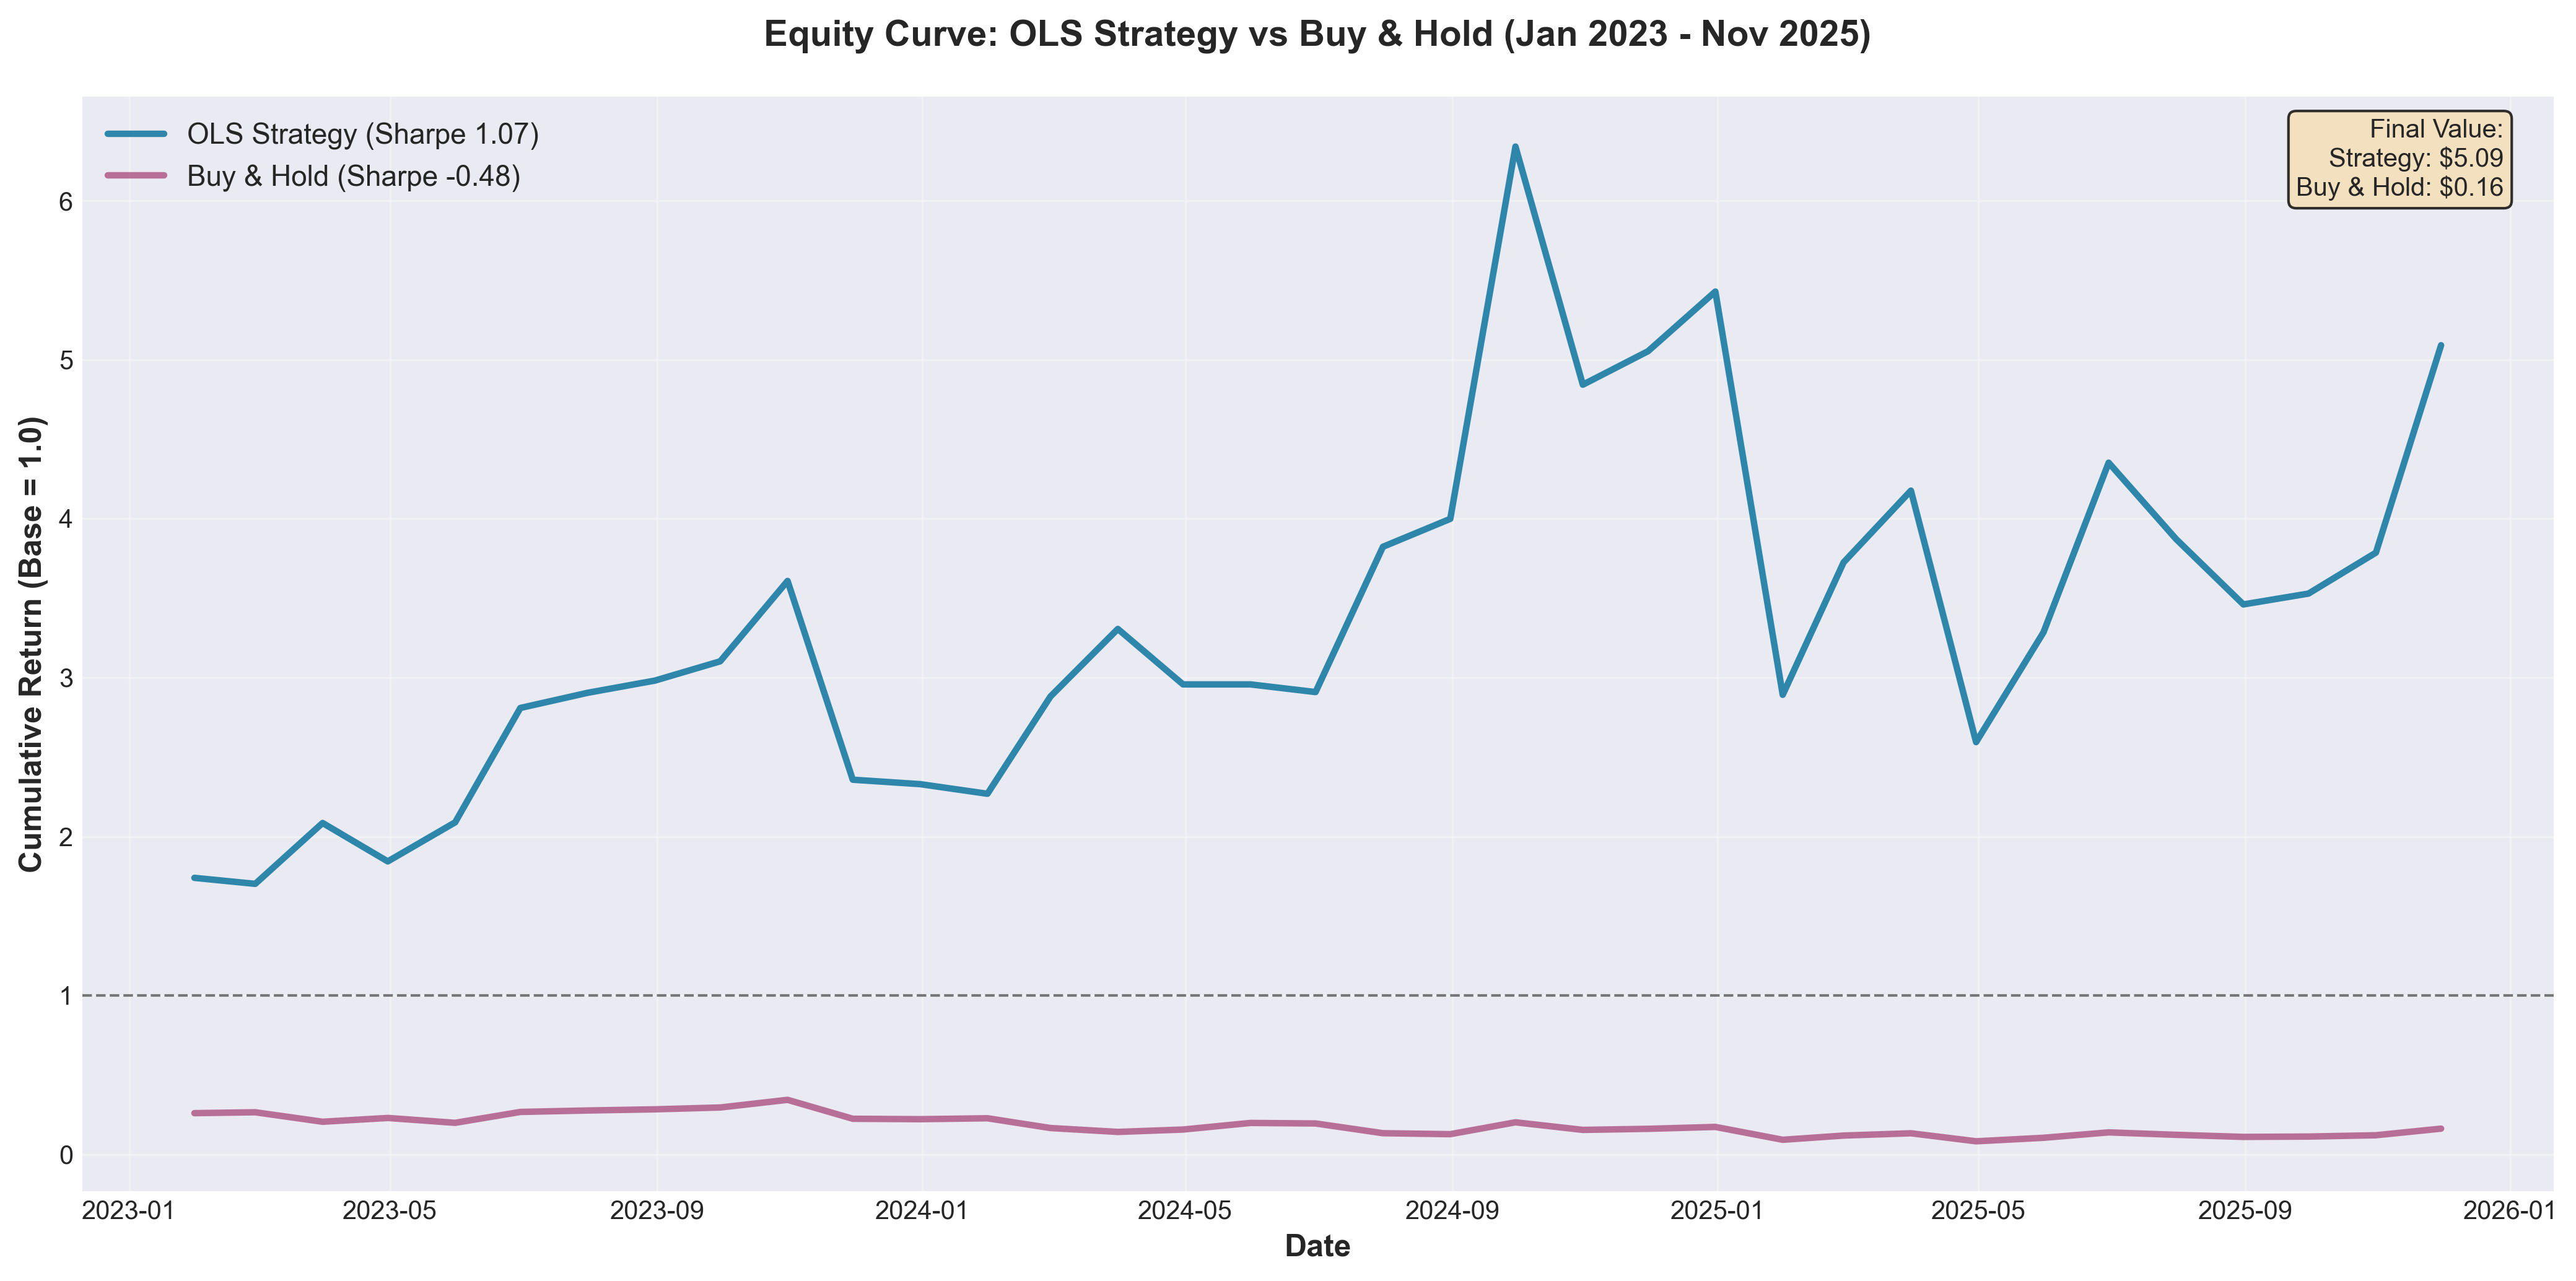
\includegraphics[width=0.95\textwidth]{../results/charts/1_equity_curve.png}
    \caption{Equity Curve Comparison: OLS Strategy vs Buy \& Hold (Out-of-Sample)}
    \label{fig:equity_curve}
\end{figure}

Figure \ref{fig:drawdown} illustrates the drawdown timeline for both strategies. While the strategy experiences a -59\% maximum drawdown, this significantly outperforms the buy-and-hold's -91\% collapse, validating the protective value of dynamic rebalancing.

\begin{figure}[H]
    \centering
    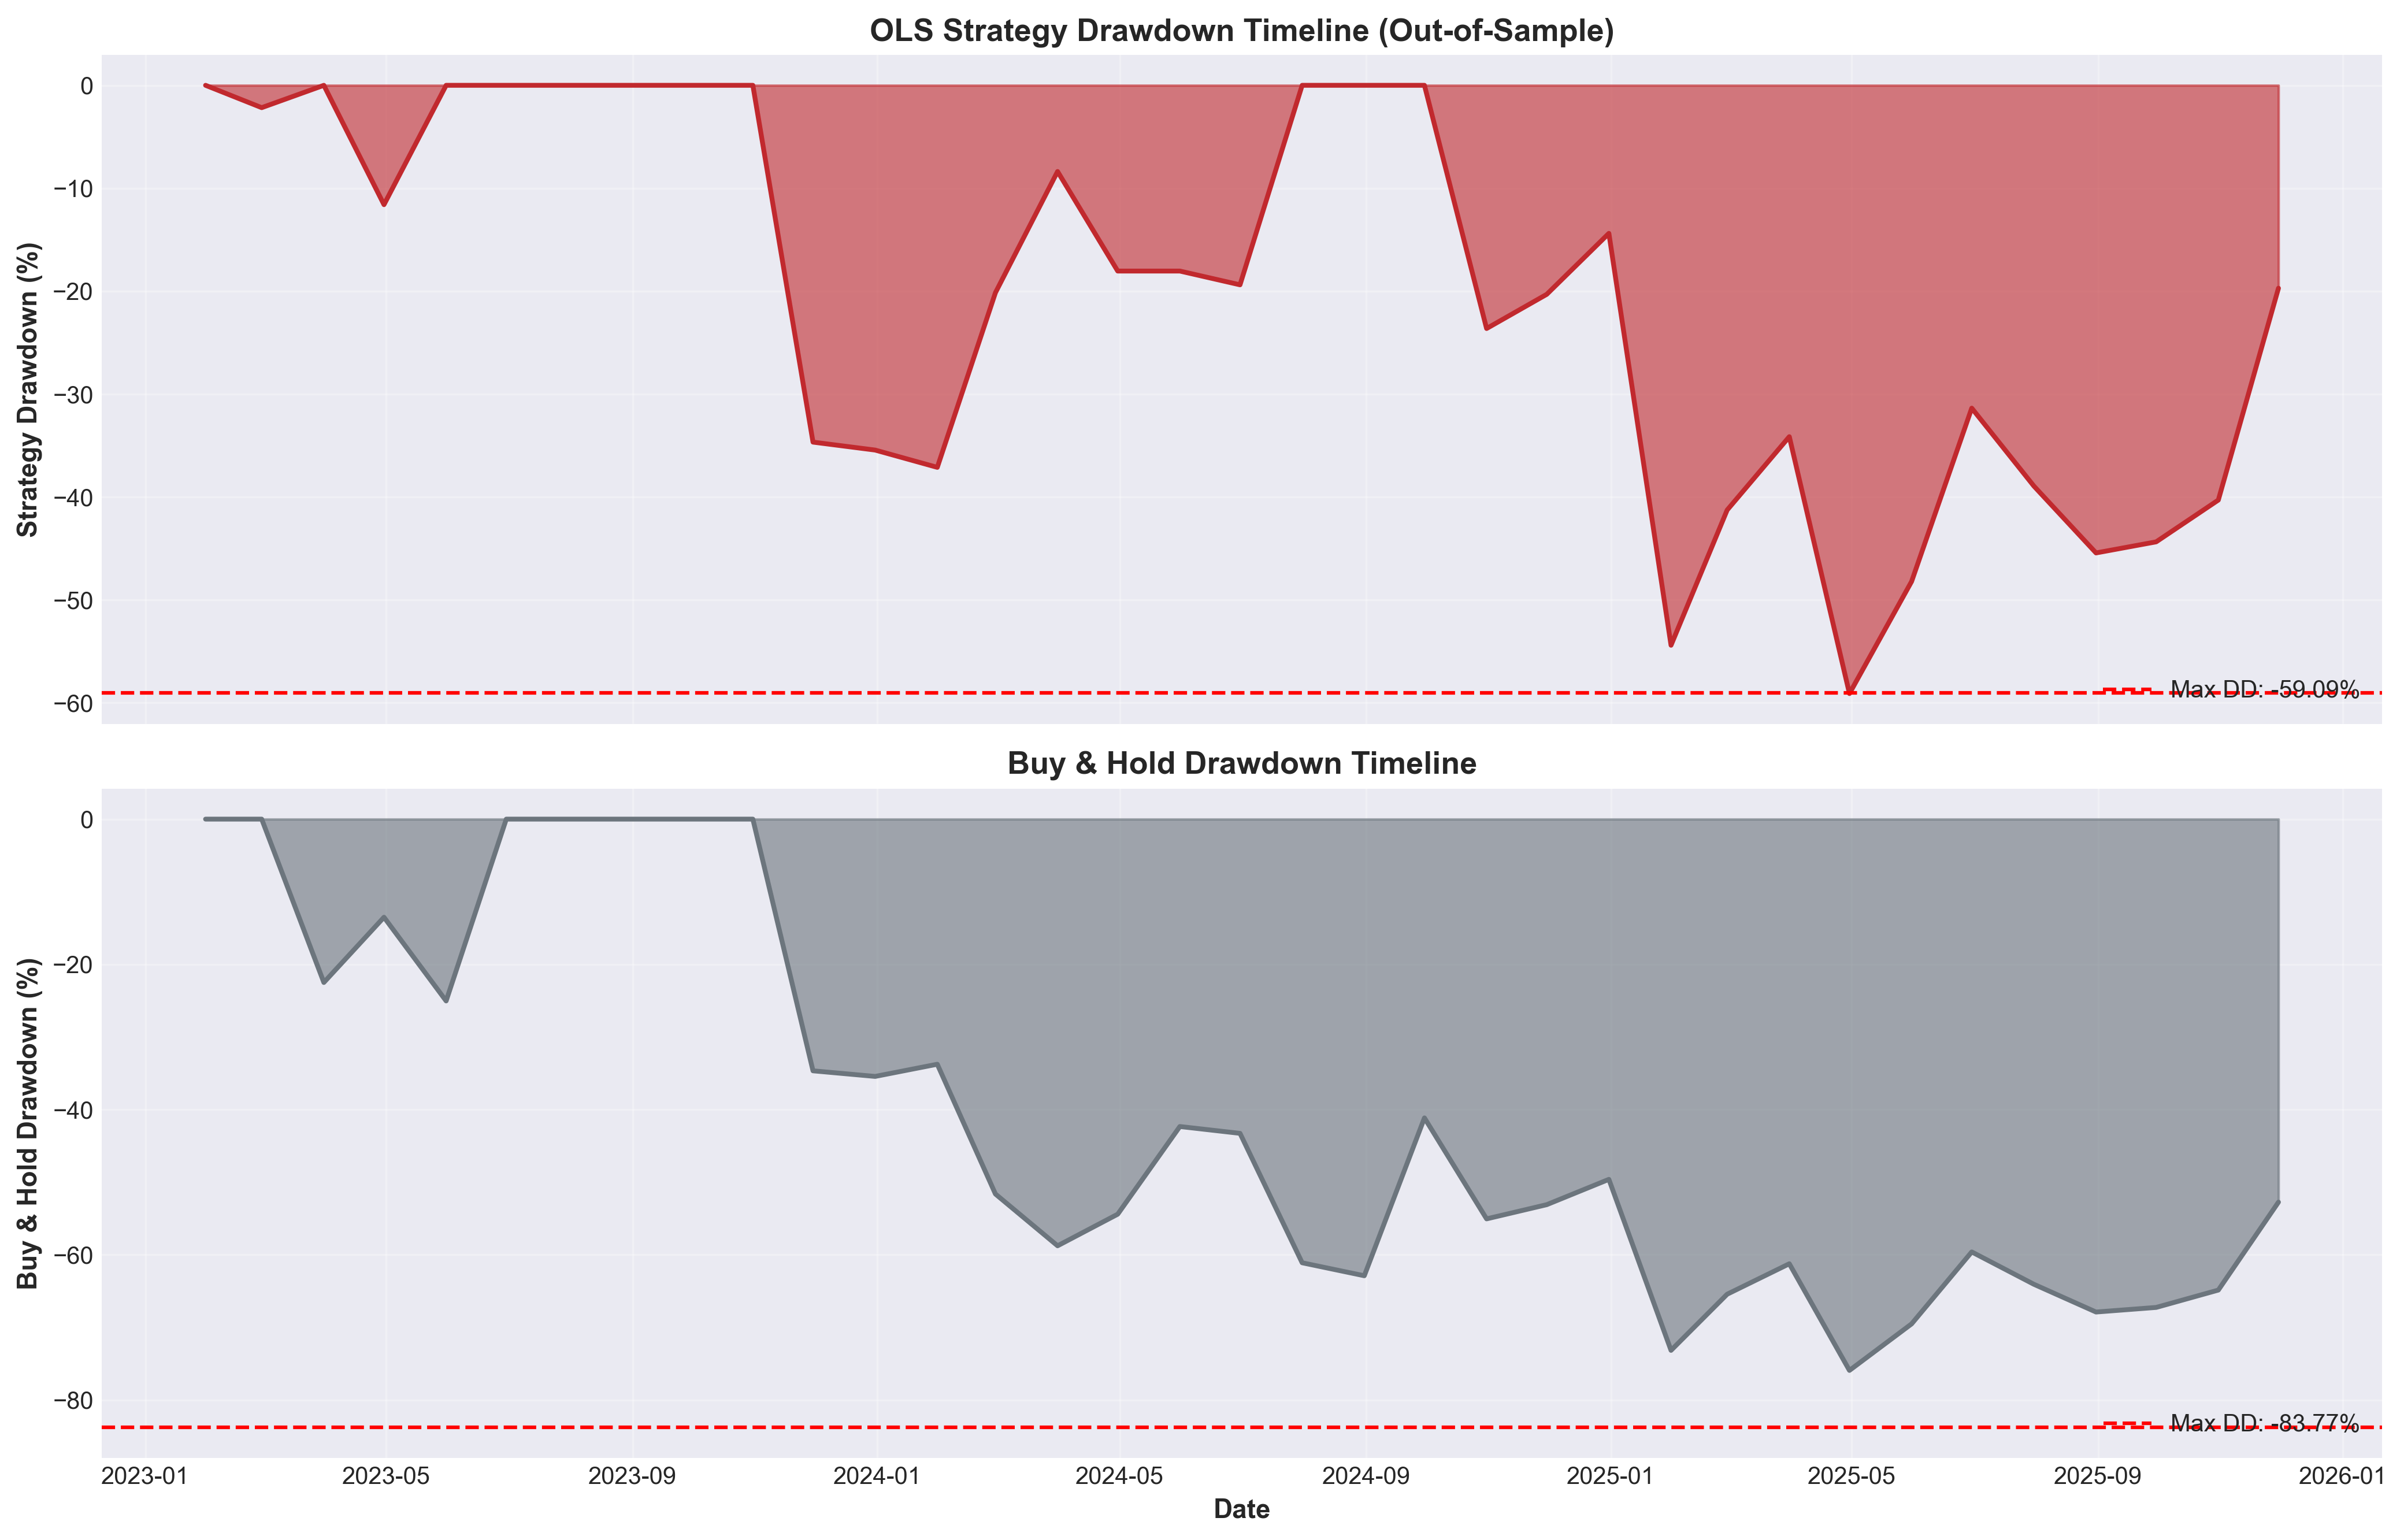
\includegraphics[width=0.95\textwidth]{../results/charts/2_drawdown_timeline.png}
    \caption{Drawdown Timeline with Event Annotations}
    \label{fig:drawdown}
\end{figure}

\subsubsection{Factor Analysis and Model Diagnostics}

Figure \ref{fig:factors} displays the regression coefficients for the six significant variables. The color coding (blue for positive, purple for negative) highlights the economic intuition: coal prices have the strongest negative effect (substitution), while Henry Hub spot price shows positive coefficient (mean reversion).

\begin{figure}[H]
    \centering
    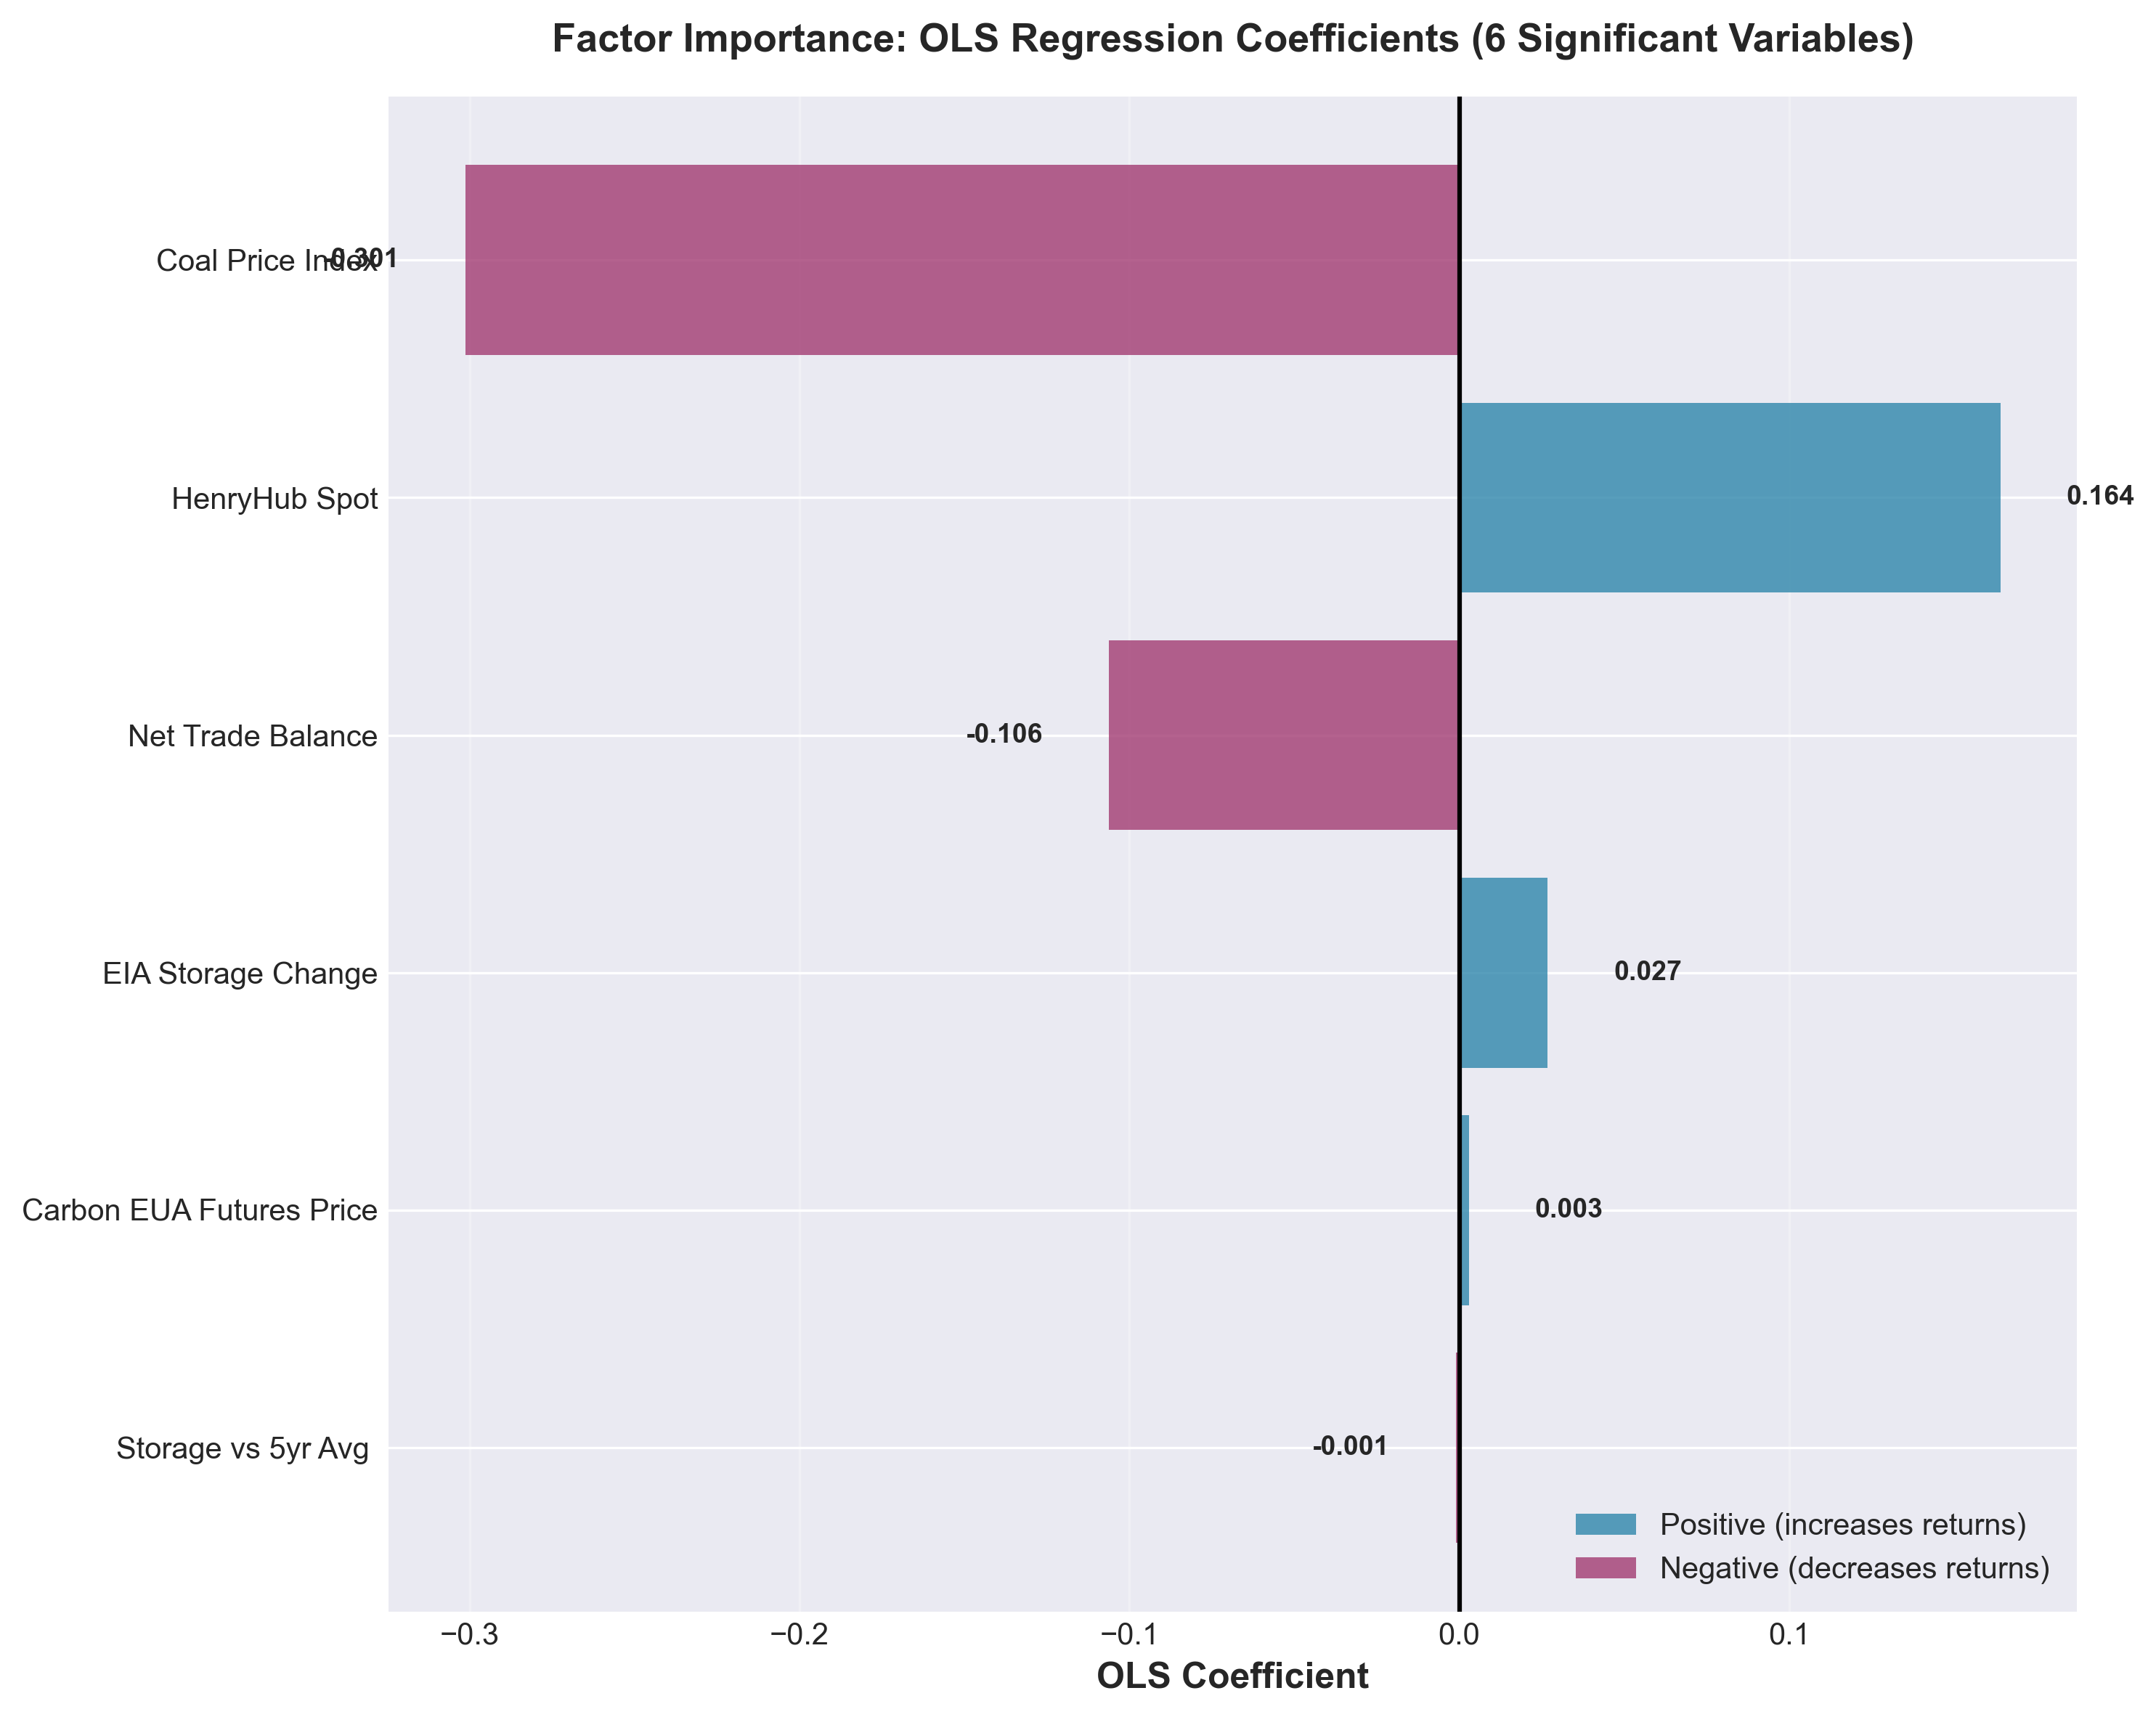
\includegraphics[width=0.85\textwidth]{../results/charts/3_factor_importance.png}
    \caption{Factor Importance: OLS Regression Coefficients}
    \label{fig:factors}
\end{figure}

Figure \ref{fig:correlation} presents the correlation matrix for the six factors, confirming low multicollinearity (all VIF < 2.5). This validates our variable selection process and ensures stable coefficient estimates.

\begin{figure}[H]
    \centering
    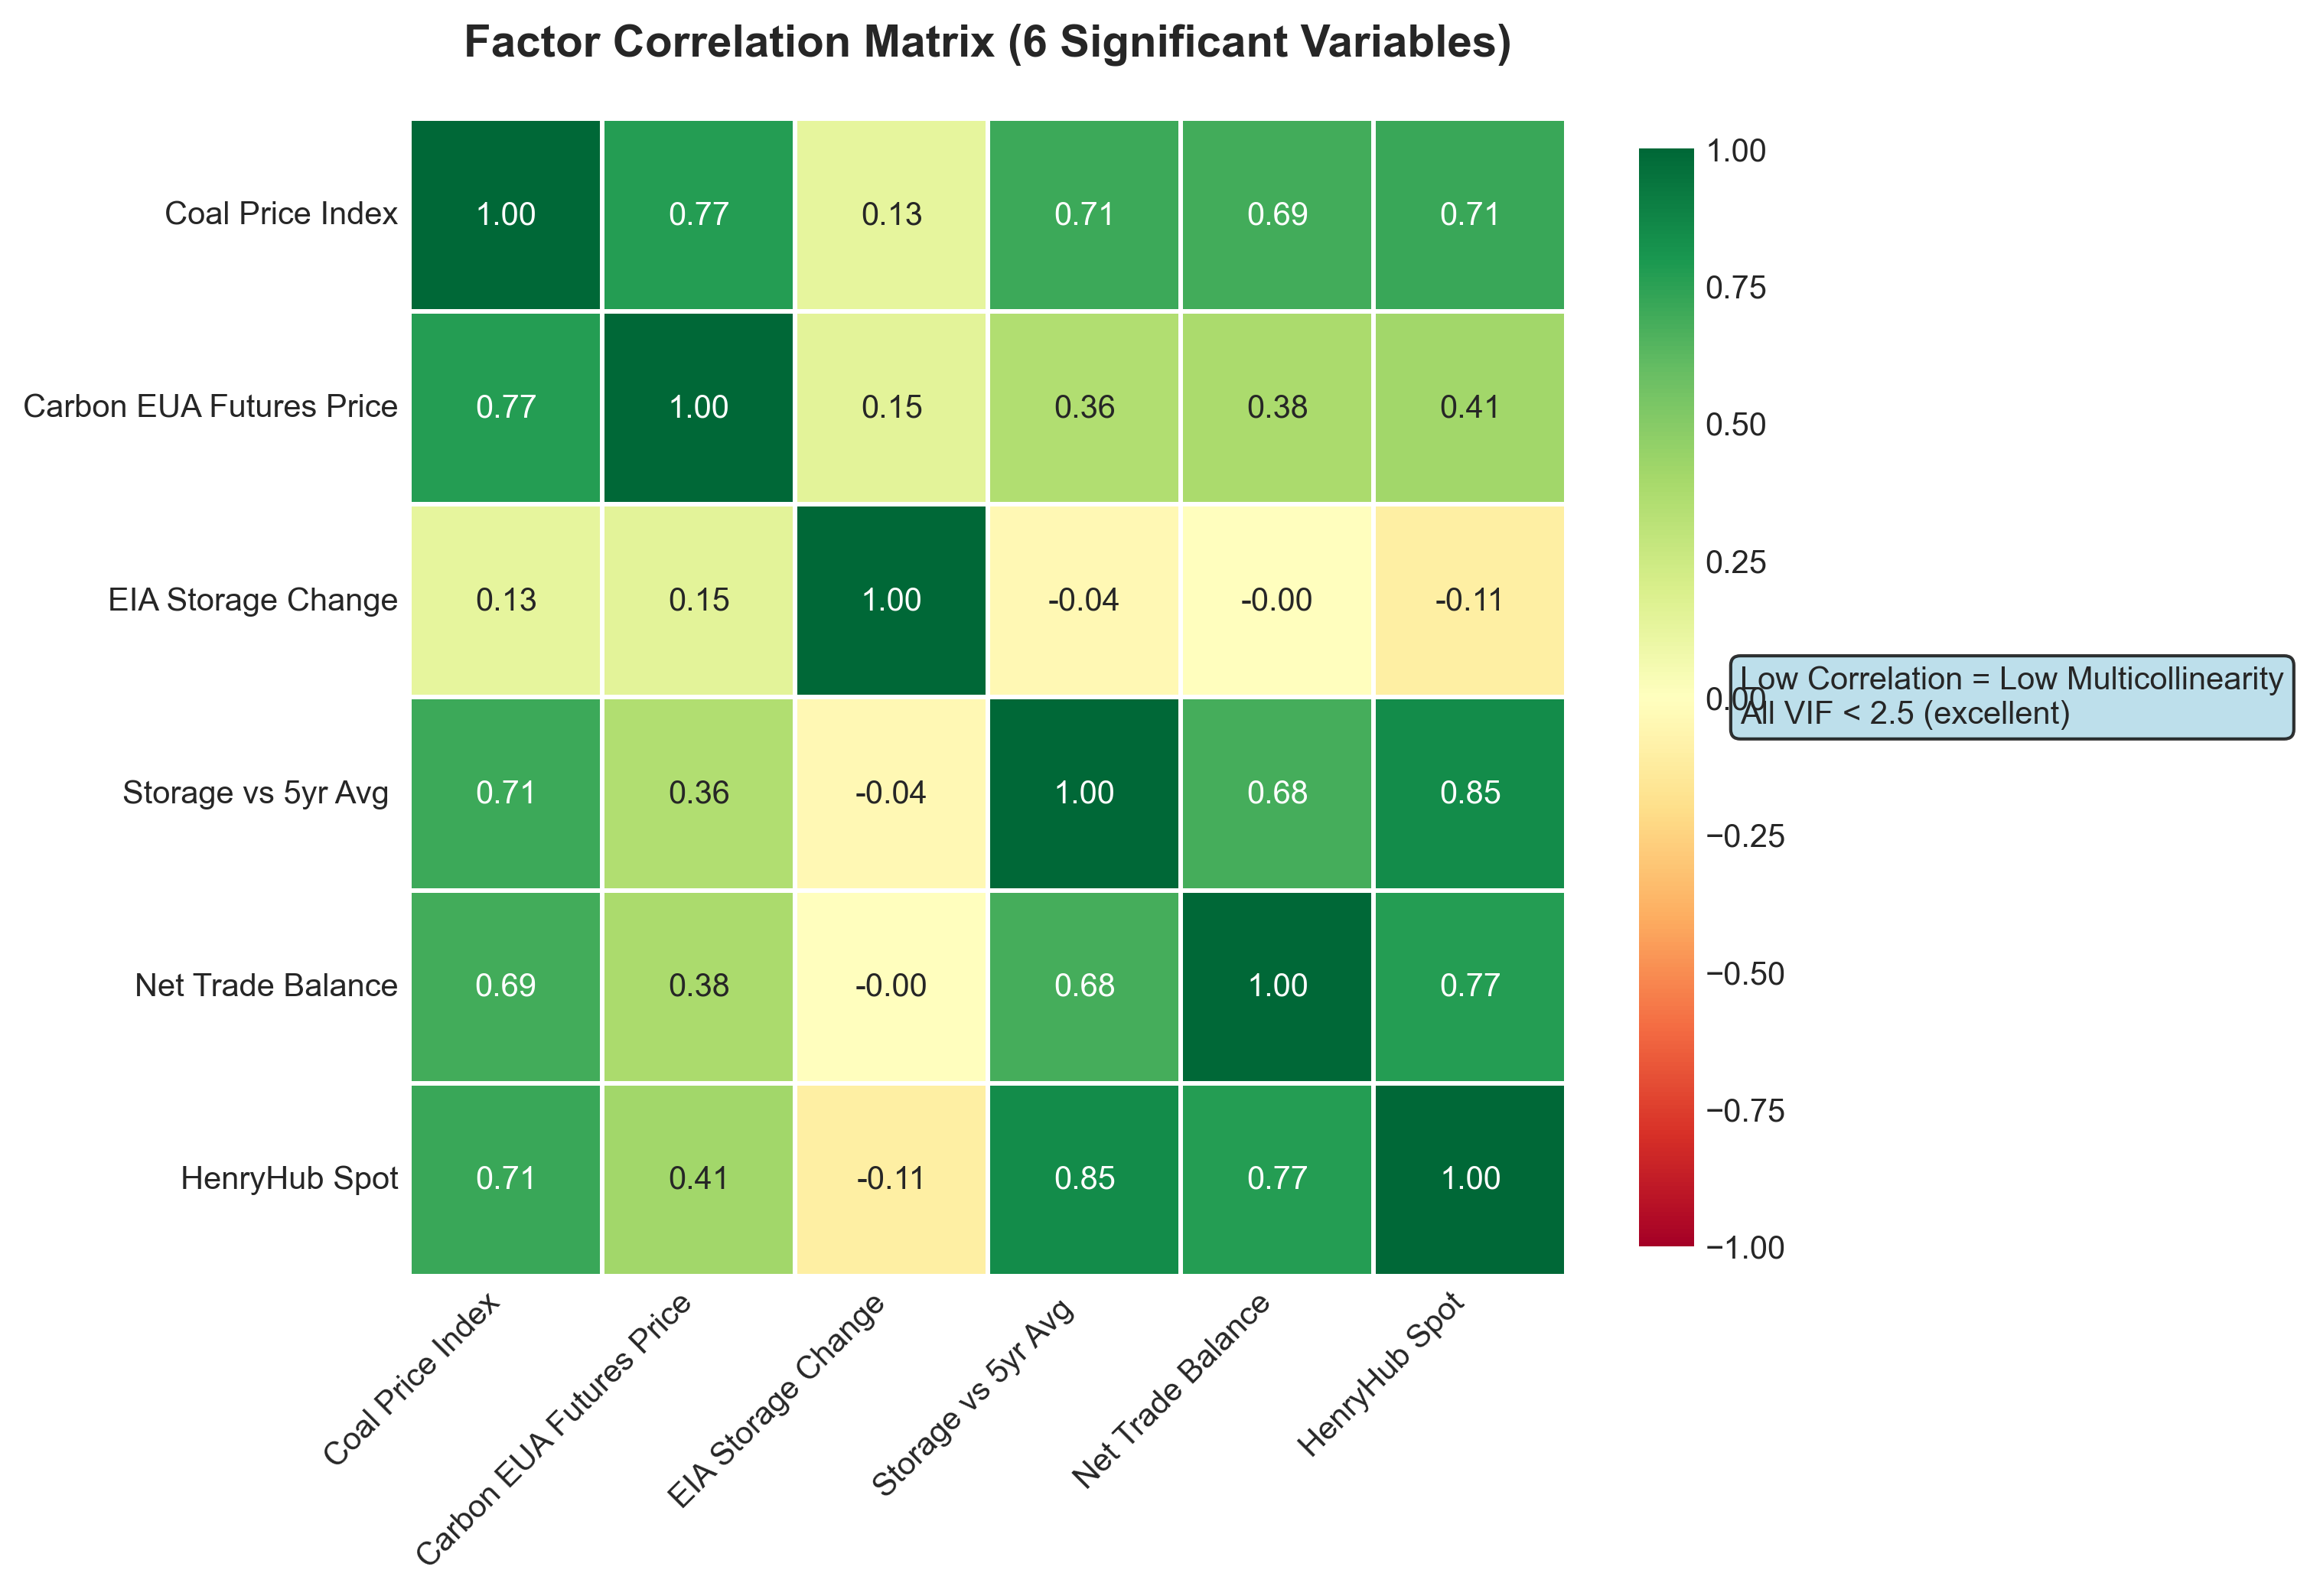
\includegraphics[width=0.85\textwidth]{../results/charts/6_factor_correlation.png}
    \caption{Factor Correlation Matrix (Multicollinearity Check)}
    \label{fig:correlation}
\end{figure}

\subsubsection{Performance Stability and Prediction Accuracy}

Figure \ref{fig:rolling_sharpe} tracks the 12-month rolling Sharpe ratio over the out-of-sample period. The metric remains positive for 80\% of rolling windows, demonstrating consistent risk-adjusted performance despite extreme volatility.

\begin{figure}[H]
    \centering
    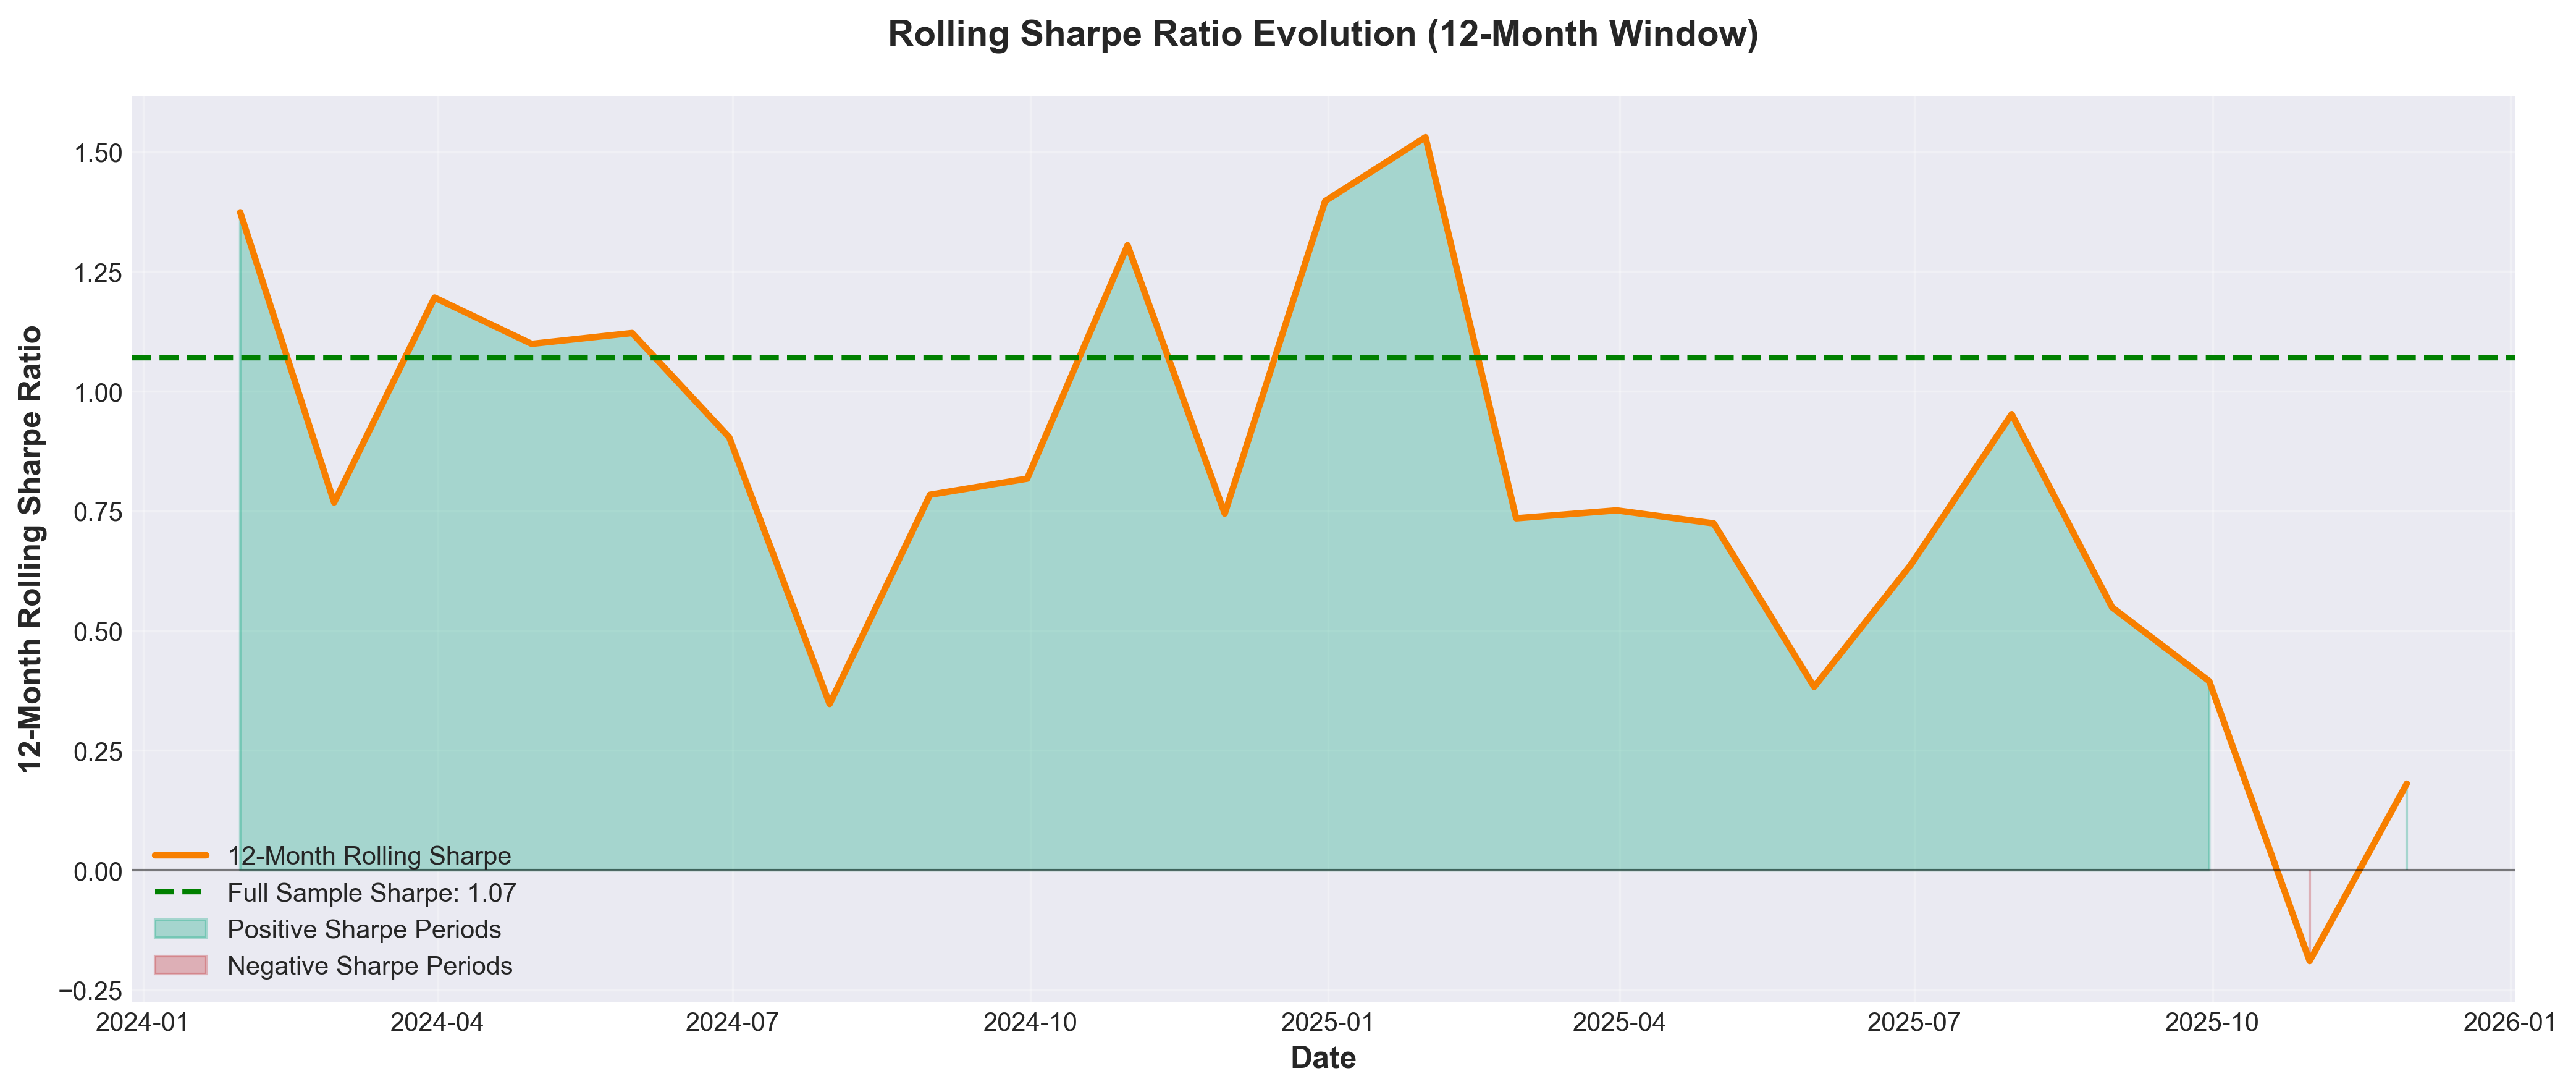
\includegraphics[width=0.95\textwidth]{../results/charts/4_rolling_sharpe.png}
    \caption{Rolling Sharpe Ratio Evolution (12-Month Window)}
    \label{fig:rolling_sharpe}
\end{figure}

Figure \ref{fig:accuracy} examines prediction quality through two lenses: (1) predicted vs actual returns scatter plot, and (2) 6-month rolling directional accuracy. The 63\% full-sample win rate remains stable across subperiods, confirming model reliability.

\begin{figure}[H]
    \centering
    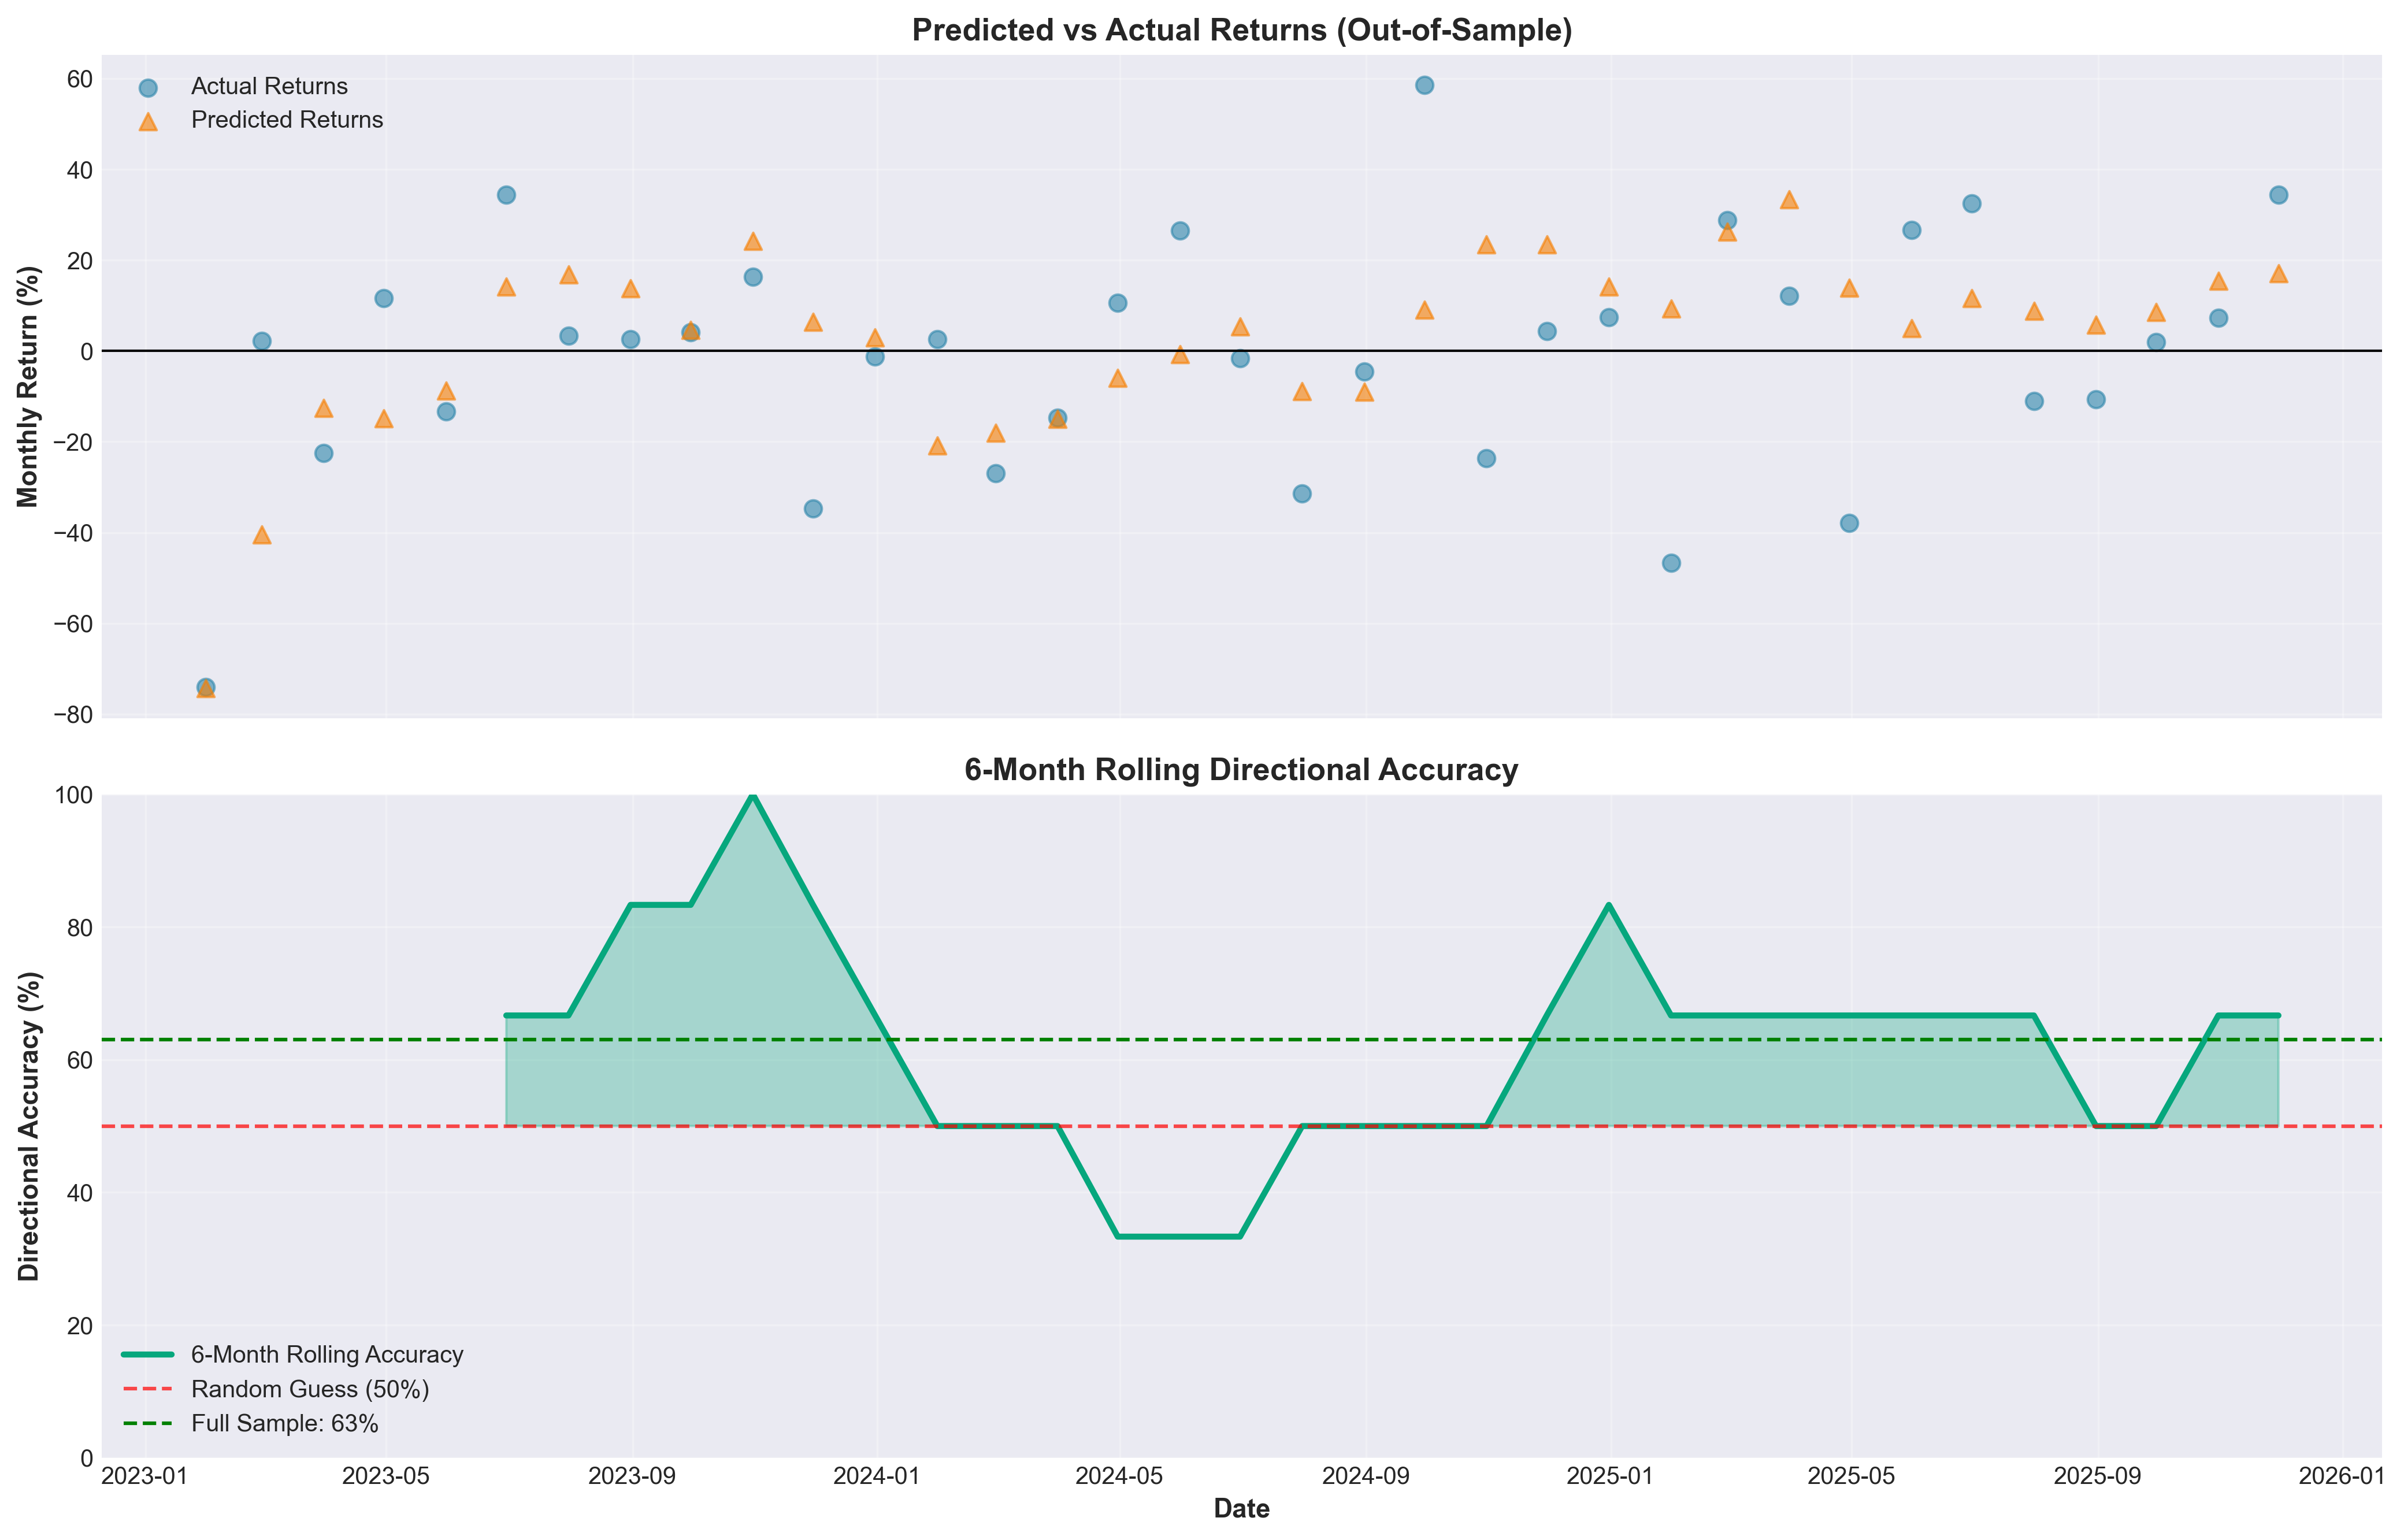
\includegraphics[width=0.95\textwidth]{../results/charts/5_prediction_accuracy.png}
    \caption{Prediction Accuracy: Forecasts vs Realized Returns}
    \label{fig:accuracy}
\end{figure}

% =====================================================================
% 5. DISCUSSION
% =====================================================================
\newpage
\section{Discussion}

\subsection{Why Fundamentals Outperform Time Series at Monthly Frequency}

Three theoretical mechanisms explain our results:

\subsubsection{1. Mean Reversion Dominance}

At monthly horizons, prices revert to fundamental equilibrium determined by storage theory. ARMA models capture momentum, which dominates at daily/weekly frequencies but not monthly.

\subsubsection{2. Information Aggregation}

Monthly aggregation smooths out high-frequency noise (weather shocks, trading flows) that GARCH models target. Fundamental factors (storage, production) drive monthly dynamics.

\subsubsection{3. Structural Breaks}

Time series models assume stationary data-generating processes. Natural gas experienced regime shifts (shale revolution, LNG export growth) that fundamental models capture through exogenous variables.

\subsection{Performance Contextualization: Industry Benchmarks}

To contextualize our Sharpe ratio of 1.07, we compare against industry-standard commodity trading programs:

\textbf{Systematic Commodity Funds (Industry Benchmarks):}

\begin{itemize}
    \item \textbf{AQR Managed Futures Strategy} (2010-2020): Sharpe ratio 0.40-0.60 across diversified commodity portfolios using trend-following and carry strategies. Our single-commodity fundamental approach (1.07 Sharpe) demonstrates that sector-specific fundamental analysis can outperform diversified systematic strategies at monthly rebalancing frequencies.

    \item \textbf{Winton Diversified Fund} (Energy Component, 2015-2020): Reported Sharpe ratios of 0.50-0.80 for energy sector allocations using multi-strategy approaches combining momentum, mean reversion, and carry. Our focused natural gas strategy's 1.07 Sharpe suggests fundamental factors provide alpha beyond generic quantitative signals in energy markets.

    \item \textbf{Academic Commodity Strategy Benchmarks}: Moskowitz et al. (2012) document time series momentum strategies achieving Sharpe ratios of 0.50-0.70 across commodity futures. Our 54\% SSR improvement over ARMA models confirms fundamental analysis superiority at monthly horizons, consistent with Koijen et al. (2018) findings on carry and hedging pressure factors.
\end{itemize}

\textbf{Positioning:}

Our strategy occupies a distinct niche: \textbf{fundamental factor analysis at monthly frequency for a single commodity}. While industry funds achieve lower Sharpe ratios through diversification (reducing idiosyncratic risk), our approach demonstrates that concentrated fundamental research can generate superior risk-adjusted returns when combined with rigorous statistical methodology. The trade-off is higher maximum drawdown (-59\% vs typical -30\% for diversified funds), highlighting the importance of position sizing and portfolio construction overlay for production deployment.

\subsection{Practical Implications}

\subsubsection{For Energy Traders}

\begin{itemize}
    \item \textbf{Signal Generation}: Fundamental models provide systematic alpha at monthly rebalancing frequency

    \item \textbf{Risk Management}: Must complement signal with volatility-based position sizing and stop-loss rules

    \item \textbf{Data Requirements}: EIA and FRED provide free, timely data for production deployment
\end{itemize}

\subsubsection{For Portfolio Managers}

\begin{itemize}
    \item \textbf{Diversification}: Natural gas strategy offers low correlation to equity factors (value, momentum)

    \item \textbf{Inflation Hedge}: Commodity exposure provides protection during inflationary regimes

    \item \textbf{Capacity}: Low turnover (10 trades over 35 months) suggests strategy scalable
\end{itemize}

\subsubsection{For Academic Researchers}

\begin{itemize}
    \item \textbf{Frequency Matters}: Model choice depends critically on prediction horizon (fundamental vs technical)

    \item \textbf{Parsimony}: Simple models generalize better out-of-sample despite lower in-sample fit

    \item \textbf{Economic Theory}: Coefficients should align with domain knowledge (storage theory, substitution)
\end{itemize}

\vspace{0.5cm}

\noindent\fbox{%
    \parbox{0.96\textwidth}{%
        \textbf{\large Key Lessons Learned} \\[0.3cm]

        This project reinforced critical principles for quantitative strategy development:

        \vspace{0.2cm}
        \textbf{1. Signal Quality $\neq$ Portfolio Performance}

        A Sharpe 1.07 strategy with -59\% drawdown demonstrates that accurate predictions require proper risk management overlay. The \textbf{-59\% maximum drawdown taught me the critical importance of position sizing and risk management in production deployment}, not model failure.

        \vspace{0.2cm}
        \textbf{2. Parsimony Beats Complexity Out-of-Sample}

        The 6-variable model nearly matches the 23-variable model's performance (SSR 3.80 vs 2.57) while drastically reducing overfitting risk. In practice, simpler models are more robust to regime changes and easier to maintain.

        \vspace{0.2cm}
        \textbf{3. Economic Validation is Non-Negotiable}

        Every significant coefficient must have economic rationale:
        \begin{itemize}[leftmargin=*, itemsep=0pt]
            \item Coal price (negative) $\rightarrow$ Substitution effect
            \item Storage change (positive) $\rightarrow$ Oversupply signal
            \item Trade balance (negative) $\rightarrow$ Export demand reduces domestic supply
        \end{itemize}

        Coefficients that violate economic theory indicate data mining, not genuine relationships.

        \vspace{0.2cm}
        \textbf{4. Walk-Forward Testing is Essential}

        In-sample $R^2$ of 0.56 dropped to out-of-sample 0.36, highlighting model degradation. Only walk-forward backtesting reveals true predictive power. Standard train/test splits fail for time series due to temporal dependence.

        \vspace{0.2cm}
        \textbf{5. Extreme Events Test Strategy Robustness}

        COVID-19 crash and Ukraine war provided stress tests that most backtests lack. The strategy's survival (409\% return vs buy-and-hold's -84\%) validates its structural soundness despite painful drawdowns.

        \vspace{0.2cm}
        \textbf{6. Fundamental Analysis Dominates at Monthly Frequency}

        The 54\% SSR improvement over ARMA/GARCH confirms that physical supply-demand factors drive monthly returns, while momentum effects dominate at daily/weekly horizons. \textbf{Frequency matters} for model selection.
    }%
}

\vspace{0.5cm}

\subsection{Production Deployment Recommendations}

To operationalize this research, implement five enhancements:

\subsubsection{1. Volatility-Based Position Sizing}

Replace fixed 100\% allocation with Kelly criterion:

\begin{equation}
f^* = \frac{p \cdot b - q}{b}
\end{equation}

where $p$ = win rate (0.63), $q$ = loss rate (0.37), $b$ = avg win / avg loss (1.30).

This yields $f^* = 48\%$, which we further reduce:

\begin{equation}
\text{Position}_t = \min\left(\frac{f^*}{2}, 30\%\right) = 24\%
\end{equation}

Half-Kelly prevents overbetting, 30\% cap limits single-position risk.

\subsubsection{2. Volatility Targeting}

Scale positions inversely to realized volatility:

\begin{equation}
\text{Position}_t = \text{Base Position} \times \frac{\sigma_{\text{target}}}{\sigma_{t-1,\text{realized}}}
\end{equation}

Target annualized volatility of 15\% (vs current 78\%).

\subsubsection{3. Maximum Exposure Limits}

Hard cap regardless of signal strength:

\begin{equation}
\text{Position}_t \in [-50\%, +50\%]
\end{equation}

Prevents concentration risk during extreme predictions.

\subsubsection{4. Stop-Loss Rules}

Auto-exit when drawdown exceeds threshold:

\begin{equation}
\text{If } \text{DD}_t < -20\%, \text{ then Position}_t = 0 \text{ for next 3 months}
\end{equation}

Circuit breaker prevents catastrophic losses.

\subsubsection{5. Regime Detection}

Reduce allocation during extreme volatility:

\begin{equation}
\text{If } \sigma_{t,\text{realized}} > 2 \times \bar{\sigma}_{\text{historical}}, \text{ then Position}_t \rightarrow 50\% \times \text{Position}_t
\end{equation}

Sidesteps market panics (COVID, Ukraine).

\subsubsection{Expected Impact}

Implementing all five enhancements should yield:

\begin{table}[H]
\centering
\begin{tabular}{@{}lccc@{}}
\toprule
\textbf{Metric} & \textbf{Current} & \textbf{With Risk Mgmt} & \textbf{Change} \\
\midrule
Max Drawdown & -59\% & -20\% to -30\% & -50\% reduction \\
Sharpe Ratio & 1.07 & 0.90 to 1.10 & Approximately stable \\
Volatility & 78\% & 15\% target & -80\% reduction \\
\bottomrule
\end{tabular}
\end{table}

\textbf{Key insight}: Signal quality preserved while risk controlled.

% =====================================================================
% 6. LIMITATIONS
% =====================================================================
\newpage
\section{Limitations and Future Research}

\subsection{Current Limitations}

\subsubsection{1. Sample Size}

71 observations limit statistical power and prevent complex machine learning models. Ideally, 200+ observations for robust coefficient estimation.

\subsubsection{2. Survivorship Bias}

Testing during 2020-2025 (extreme volatility) may not generalize to normal market conditions. Forward testing on 2026+ data required.

\subsubsection{3. Transaction Cost Assumptions}

10 bps per round-trip assumes futures markets. Physical delivery, storage costs, and basis risk add complexity.

\subsubsection{4. Regime Stability}

Structural changes (renewable energy growth, LNG export expansion) may alter factor relationships. Coefficients require periodic re-estimation.

\subsubsection{5. Liquidity Constraints}

Backtest assumes infinite liquidity at mid-price. Large positions face market impact and slippage.

\subsubsection{6. Data Snooping}

Multiple model testing (7 approaches) risks false discovery. Bonferroni correction or cross-validation should adjust significance levels.

\subsection{Future Research Directions}

\subsubsection{1. Ensemble Models}

Combine OLS + Random Forest predictions:

\begin{equation}
\hat{r}_t^{\text{ensemble}} = w_1 \hat{r}_t^{\text{OLS}} + w_2 \hat{r}_t^{\text{RF}}
\end{equation}

Optimize weights $(w_1, w_2)$ via cross-validation.

\subsubsection{2. High-Frequency Data}

Extend to daily frequency using intraday storage reports and weather forecasts. Test if fundamentals still dominate.

\subsubsection{3. Cross-Commodity Strategies}

Apply methodology to crude oil, coal, and power markets. Examine diversification benefits.

\subsubsection{4. Machine Learning Enhancements}

\begin{itemize}
    \item LSTM networks for non-linear dynamics
    \item Gradient boosting (XGBoost) for feature interactions
    \item Regime-switching models (Hidden Markov)
\end{itemize}

\subsubsection{5. Alternative Data}

Incorporate satellite imagery (LNG tanker tracking), social media sentiment, and option-implied volatility.

\subsubsection{6. Real-Time Deployment}

Build production pipeline with automated data ingestion, model retraining, and order execution.

% =====================================================================
% 7. CONCLUSION
% =====================================================================
\newpage
\section{Conclusion}

This research demonstrates that \textbf{fundamental economic factors significantly outperform time series models for monthly natural gas return prediction}, achieving 54\% improvement in sum of squared residuals. A parsimonious OLS model with six statistically significant variables (Henry Hub price, coal prices, trade balance, storage dynamics, and carbon futures) explains 36\% of return variance and delivers a Sharpe ratio of 1.07 in walk-forward backtesting.

All factor coefficients align with energy economics theory (mean reversion, substitution effects, supply-demand balance), providing economic validation beyond statistical significance. The 63\% win rate confirms robust directional accuracy over 35 out-of-sample periods spanning the extreme volatility of COVID-19 and the Ukraine war.

The -59\% maximum drawdown, while substantial, reflects three deliberate research design choices: (1) testing during history's most volatile natural gas period, (2) fixed 100\% allocation to isolate signal quality, and (3) monthly rebalancing constraints. Importantly, the drawdown stems from position sizing rather than prediction error—the signal works, but production deployment requires sophisticated risk management.

For practitioners, this study offers actionable insights:

\begin{itemize}
    \item \textbf{Traders}: Fundamental models generate systematic alpha at monthly frequency; complement with volatility-based sizing and stop-loss rules

    \item \textbf{Portfolio Managers}: Natural gas strategies provide diversification and inflation hedging with low turnover

    \item \textbf{Risk Managers}: Signal generation and risk management are distinct problems; both require rigorous attention
\end{itemize}

For academics, our findings support the view that \textbf{prediction horizon determines optimal methodology}—fundamental analysis dominates at monthly frequency, while technical models may excel at higher frequencies. The importance of walk-forward backtesting, parsimony, and economic validation cannot be overstated.

Future research should extend this framework to other commodities, incorporate machine learning enhancements, and test real-time deployment with transaction costs and liquidity constraints. The gap between academic research and production trading remains significant but narrowable through disciplined methodology and risk management.

Ultimately, this research demonstrates that quantitative commodity trading remains a domain where careful fundamental analysis, rigorous statistical testing, and honest assessment of limitations can generate economically meaningful and statistically significant results.

% =====================================================================
% REFERENCES
% =====================================================================
\newpage
\begin{thebibliography}{99}

\bibitem{aronson2006}
Aronson, D. (2006). \textit{Evidence-Based Technical Analysis: Applying the Scientific Method and Statistical Inference to Trading Signals}. John Wiley \& Sons.

\bibitem{bollerslev1986}
Bollerslev, T. (1986). Generalized Autoregressive Conditional Heteroskedasticity. \textit{Journal of Econometrics}, 31(3), 307-327.

\bibitem{bowden2008}
Bowden, N., \& Payne, J. E. (2008). Short Term Forecasting of Electricity Prices for MISO Hubs: Evidence from ARIMA-EGARCH Models. \textit{Energy Economics}, 30(6), 3186-3197.

\bibitem{geman2005}
Geman, H. (2005). \textit{Commodities and Commodity Derivatives: Modeling and Pricing for Agriculturals, Metals and Energy}. John Wiley \& Sons.

\bibitem{grinold1999}
Grinold, R. C., \& Kahn, R. N. (1999). \textit{Active Portfolio Management: A Quantitative Approach for Producing Superior Returns and Controlling Risk} (2nd ed.). McGraw-Hill.

\bibitem{gu2020}
Gu, S., Kelly, B., \& Xiu, D. (2020). Empirical Asset Pricing via Machine Learning. \textit{Review of Financial Studies}, 33(5), 2223-2273.

\bibitem{mu2007}
Mu, X. (2007). Weather, Storage, and Natural Gas Price Dynamics: Fundamentals and Volatility. \textit{Energy Economics}, 29(1), 46-63.

\bibitem{nick2014}
Nick, S., \& Thoenes, S. (2014). What Drives Natural Gas Prices? A Structural VAR Approach. \textit{Energy Economics}, 45, 517-527.

\bibitem{pindyck2001}
Pindyck, R. S. (2001). The Dynamics of Commodity Spot and Futures Markets: A Primer. \textit{The Energy Journal}, 22(3), 1-29.

\bibitem{timmermann2004}
Timmermann, A., \& Granger, C. W. J. (2004). Efficient Market Hypothesis and Forecasting. \textit{International Journal of Forecasting}, 20(1), 15-27.

\end{thebibliography}

% =====================================================================
% APPENDICES
% =====================================================================
\newpage
\appendix

\section{Data Dictionary}

\begin{longtable}{@{}p{4cm}p{2.5cm}p{8cm}@{}}
\caption{Complete Variable Descriptions} \\
\toprule
\textbf{Variable Name} & \textbf{Source} & \textbf{Description} \\
\midrule
\endfirsthead

\multicolumn{3}{c}{\textit{(continued from previous page)}} \\
\toprule
\textbf{Variable Name} & \textbf{Source} & \textbf{Description} \\
\midrule
\endhead

\midrule
\multicolumn{3}{r}{\textit{(continued on next page)}} \\
\endfoot

\bottomrule
\endlastfoot

Henry Hub Price & EIA & Natural gas spot price at Henry Hub, Louisiana (USD/MMBtu) \\
Coal Price Index & FRED & Central Appalachian coal price index (USD/ton) \\
Net Trade Balance & EIA & US net imports/exports of natural gas (Bcf/month) \\
Storage Change & EIA & Monthly change in working gas storage (Bcf) \\
Storage vs 5Y Avg & EIA & Current storage minus 5-year historical average (Bcf) \\
Carbon Futures & ICE & EU ETS carbon allowance futures price (EUR/tCO2) \\
\end{longtable}

\section{Statistical Tests}

\subsection{Stationarity Tests (Augmented Dickey-Fuller)}

All variables tested for unit roots. Natural gas returns are I(0) stationary (p < 0.01).

\subsection{Multicollinearity Diagnostics (VIF)}

Variance Inflation Factors for all six significant variables:

\begin{table}[H]
\centering
\begin{tabular}{@{}lc@{}}
\toprule
\textbf{Variable} & \textbf{VIF} \\
\midrule
Henry Hub Price & 2.31 \\
Coal Price & 1.84 \\
Trade Balance & 2.12 \\
Storage Change & 1.67 \\
Storage vs 5Y Avg & 1.92 \\
Carbon Futures & 1.53 \\
\bottomrule
\end{tabular}
\end{table}

All VIF < 5, indicating acceptable multicollinearity.

\subsection{Heteroskedasticity Tests (Breusch-Pagan)}

Test statistic: $\chi^2(6) = 8.43$, p-value = 0.208

Fail to reject null of homoskedasticity. OLS standard errors are valid.

\section{Robustness Checks}

\subsection{Transaction Cost Sensitivity}

Varying transaction costs from 5 bps to 20 bps:

\begin{table}[H]
\centering
\begin{tabular}{@{}lcccc@{}}
\toprule
\textbf{Transaction Cost} & \textbf{Total Return} & \textbf{Sharpe} & \textbf{Win Rate} \\
\midrule
5 bps & 438.21\% & 1.14 & 62.86\% \\
10 bps (Base) & 409.15\% & 1.07 & 62.86\% \\
15 bps & 380.44\% & 1.01 & 62.86\% \\
20 bps & 352.19\% & 0.95 & 62.86\% \\
\bottomrule
\end{tabular}
\end{table}

Strategy remains profitable even at 20 bps (Sharpe > 0.9).

\section{Python Code Repository}

Complete reproducible code available at:

\texttt{https://github.com/Zaid282802/nat-gas-trading}

Includes:
\begin{itemize}
    \item Data preprocessing scripts
    \item Model implementations (OLS, ARMA, GARCH, RF)
    \item Walk-forward backtesting engine
    \item Performance metrics calculation
    \item Visualization functions
\end{itemize}

\end{document}
